% Options for packages loaded elsewhere
% Options for packages loaded elsewhere
\PassOptionsToPackage{unicode}{hyperref}
\PassOptionsToPackage{hyphens}{url}
%
\documentclass[
  spanish,
  11.5pt,
  170mm x 240mmpaper,
]{scrbook}
\usepackage{xcolor}
\usepackage[left=3.5cm,right=3.5cm,top=3.5cm,bottom=3.5cm]{geometry}
\usepackage{amsmath,amssymb}
\setcounter{secnumdepth}{5}
\usepackage{iftex}
\ifPDFTeX
  \usepackage[T1]{fontenc}
  \usepackage[utf8]{inputenc}
  \usepackage{textcomp} % provide euro and other symbols
\else % if luatex or xetex
  \usepackage{unicode-math} % this also loads fontspec
  \defaultfontfeatures{Scale=MatchLowercase}
  \defaultfontfeatures[\rmfamily]{Ligatures=TeX,Scale=1}
\fi
\usepackage{lmodern}
\ifPDFTeX\else
  % xetex/luatex font selection
\fi
% Use upquote if available, for straight quotes in verbatim environments
\IfFileExists{upquote.sty}{\usepackage{upquote}}{}
\IfFileExists{microtype.sty}{% use microtype if available
  \usepackage[]{microtype}
  \UseMicrotypeSet[protrusion]{basicmath} % disable protrusion for tt fonts
}{}
\makeatletter
\@ifundefined{KOMAClassName}{% if non-KOMA class
  \IfFileExists{parskip.sty}{%
    \usepackage{parskip}
  }{% else
    \setlength{\parindent}{0pt}
    \setlength{\parskip}{6pt plus 2pt minus 1pt}}
}{% if KOMA class
  \KOMAoptions{parskip=half}}
\makeatother
% Make \paragraph and \subparagraph free-standing
\makeatletter
\ifx\paragraph\undefined\else
  \let\oldparagraph\paragraph
  \renewcommand{\paragraph}{
    \@ifstar
      \xxxParagraphStar
      \xxxParagraphNoStar
  }
  \newcommand{\xxxParagraphStar}[1]{\oldparagraph*{#1}\mbox{}}
  \newcommand{\xxxParagraphNoStar}[1]{\oldparagraph{#1}\mbox{}}
\fi
\ifx\subparagraph\undefined\else
  \let\oldsubparagraph\subparagraph
  \renewcommand{\subparagraph}{
    \@ifstar
      \xxxSubParagraphStar
      \xxxSubParagraphNoStar
  }
  \newcommand{\xxxSubParagraphStar}[1]{\oldsubparagraph*{#1}\mbox{}}
  \newcommand{\xxxSubParagraphNoStar}[1]{\oldsubparagraph{#1}\mbox{}}
\fi
\makeatother


\usepackage{longtable,booktabs,array}
\newcounter{none} % for unnumbered tables
\usepackage{calc} % for calculating minipage widths
% Correct order of tables after \paragraph or \subparagraph
\usepackage{etoolbox}
\makeatletter
\patchcmd\longtable{\par}{\if@noskipsec\mbox{}\fi\par}{}{}
\makeatother
% Allow footnotes in longtable head/foot
\IfFileExists{footnotehyper.sty}{\usepackage{footnotehyper}}{\usepackage{footnote}}
\makesavenoteenv{longtable}
\usepackage{graphicx}
\makeatletter
\newsavebox\pandoc@box
\newcommand*\pandocbounded[1]{% scales image to fit in text height/width
  \sbox\pandoc@box{#1}%
  \Gscale@div\@tempa{\textheight}{\dimexpr\ht\pandoc@box+\dp\pandoc@box\relax}%
  \Gscale@div\@tempb{\linewidth}{\wd\pandoc@box}%
  \ifdim\@tempb\p@<\@tempa\p@\let\@tempa\@tempb\fi% select the smaller of both
  \ifdim\@tempa\p@<\p@\scalebox{\@tempa}{\usebox\pandoc@box}%
  \else\usebox{\pandoc@box}%
  \fi%
}
% Set default figure placement to htbp
\def\fps@figure{htbp}
\makeatother


% definitions for citeproc citations
\NewDocumentCommand\citeproctext{}{}
\NewDocumentCommand\citeproc{mm}{%
  \begingroup\def\citeproctext{#2}\cite{#1}\endgroup}
\makeatletter
 % allow citations to break across lines
 \let\@cite@ofmt\@firstofone
 % avoid brackets around text for \cite:
 \def\@biblabel#1{}
 \def\@cite#1#2{{#1\if@tempswa , #2\fi}}
\makeatother
\newlength{\cslhangindent}
\setlength{\cslhangindent}{1.5em}
\newlength{\csllabelwidth}
\setlength{\csllabelwidth}{3em}
\newenvironment{CSLReferences}[2] % #1 hanging-indent, #2 entry-spacing
 {\begin{list}{}{%
  \setlength{\itemindent}{0pt}
  \setlength{\leftmargin}{0pt}
  \setlength{\parsep}{0pt}
  % turn on hanging indent if param 1 is 1
  \ifodd #1
   \setlength{\leftmargin}{\cslhangindent}
   \setlength{\itemindent}{-1\cslhangindent}
  \fi
  % set entry spacing
  \setlength{\itemsep}{#2\baselineskip}}}
 {\end{list}}
\usepackage{calc}
\newcommand{\CSLBlock}[1]{\hfill\break\parbox[t]{\linewidth}{\strut\ignorespaces#1\strut}}
\newcommand{\CSLLeftMargin}[1]{\parbox[t]{\csllabelwidth}{\strut#1\strut}}
\newcommand{\CSLRightInline}[1]{\parbox[t]{\linewidth - \csllabelwidth}{\strut#1\strut}}
\newcommand{\CSLIndent}[1]{\hspace{\cslhangindent}#1}

\ifLuaTeX
\usepackage[bidi=basic,shorthands=off]{babel}
\else
\usepackage[bidi=default,shorthands=off]{babel}
\fi
\ifLuaTeX
  \usepackage{selnolig} % disable illegal ligatures
\fi


\setlength{\emergencystretch}{3em} % prevent overfull lines

\providecommand{\tightlist}{%
  \setlength{\itemsep}{0pt}\setlength{\parskip}{0pt}}



 


\usepackage{setspace}
\setstretch{1.5}                     % Interlineado del cuerpo (reemplaza spacing: 1.5)
\addtokomafont{disposition}{\linespread{1.2}\selectfont} % Títulos con interlineado estándar
\usepackage{fontspec}
\setmainfont{Roboto}
\usepackage{microtype}
\setlength{\parindent}{0pt}
\setlength{\parskip}{1.2em}
\pretolerance=100
\tolerance=200
\emergencystretch=3em
\hyphenpenalty=50
\exhyphenpenalty=50
\RedeclareSectionCommand[afterskip=0.5\baselineskip]{chapter}
\makeatletter
\@ifpackageloaded{bookmark}{}{\usepackage{bookmark}}
\makeatother
\makeatletter
\@ifpackageloaded{caption}{}{\usepackage{caption}}
\AtBeginDocument{%
\ifdefined\contentsname
  \renewcommand*\contentsname{Tabla de contenidos}
\else
  \newcommand\contentsname{Tabla de contenidos}
\fi
\ifdefined\listfigurename
  \renewcommand*\listfigurename{Listado de Figuras}
\else
  \newcommand\listfigurename{Listado de Figuras}
\fi
\ifdefined\listtablename
  \renewcommand*\listtablename{Listado de Tablas}
\else
  \newcommand\listtablename{Listado de Tablas}
\fi
\ifdefined\figurename
  \renewcommand*\figurename{Figura}
\else
  \newcommand\figurename{Figura}
\fi
\ifdefined\tablename
  \renewcommand*\tablename{Tabla}
\else
  \newcommand\tablename{Tabla}
\fi
}
\@ifpackageloaded{float}{}{\usepackage{float}}
\floatstyle{ruled}
\@ifundefined{c@chapter}{\newfloat{codelisting}{h}{lop}}{\newfloat{codelisting}{h}{lop}[chapter]}
\floatname{codelisting}{Listado}
\newcommand*\listoflistings{\listof{codelisting}{Listado de Listados}}
\makeatother
\makeatletter
\makeatother
\makeatletter
\@ifpackageloaded{caption}{}{\usepackage{caption}}
\@ifpackageloaded{subcaption}{}{\usepackage{subcaption}}
\makeatother
\usepackage{bookmark}
\IfFileExists{xurl.sty}{\usepackage{xurl}}{} % add URL line breaks if available
\urlstyle{same}
\hypersetup{
  pdflang={es},
  hidelinks,
  pdfcreator={LaTeX via pandoc}}


\author{}
\date{}
\begin{document}
\frontmatter

% ============================================
% PÁGINA 1: PORTADA COMPLETA
% ============================================
\begin{titlepage}
    \thispagestyle{empty}
    \pagestyle{empty}
    
        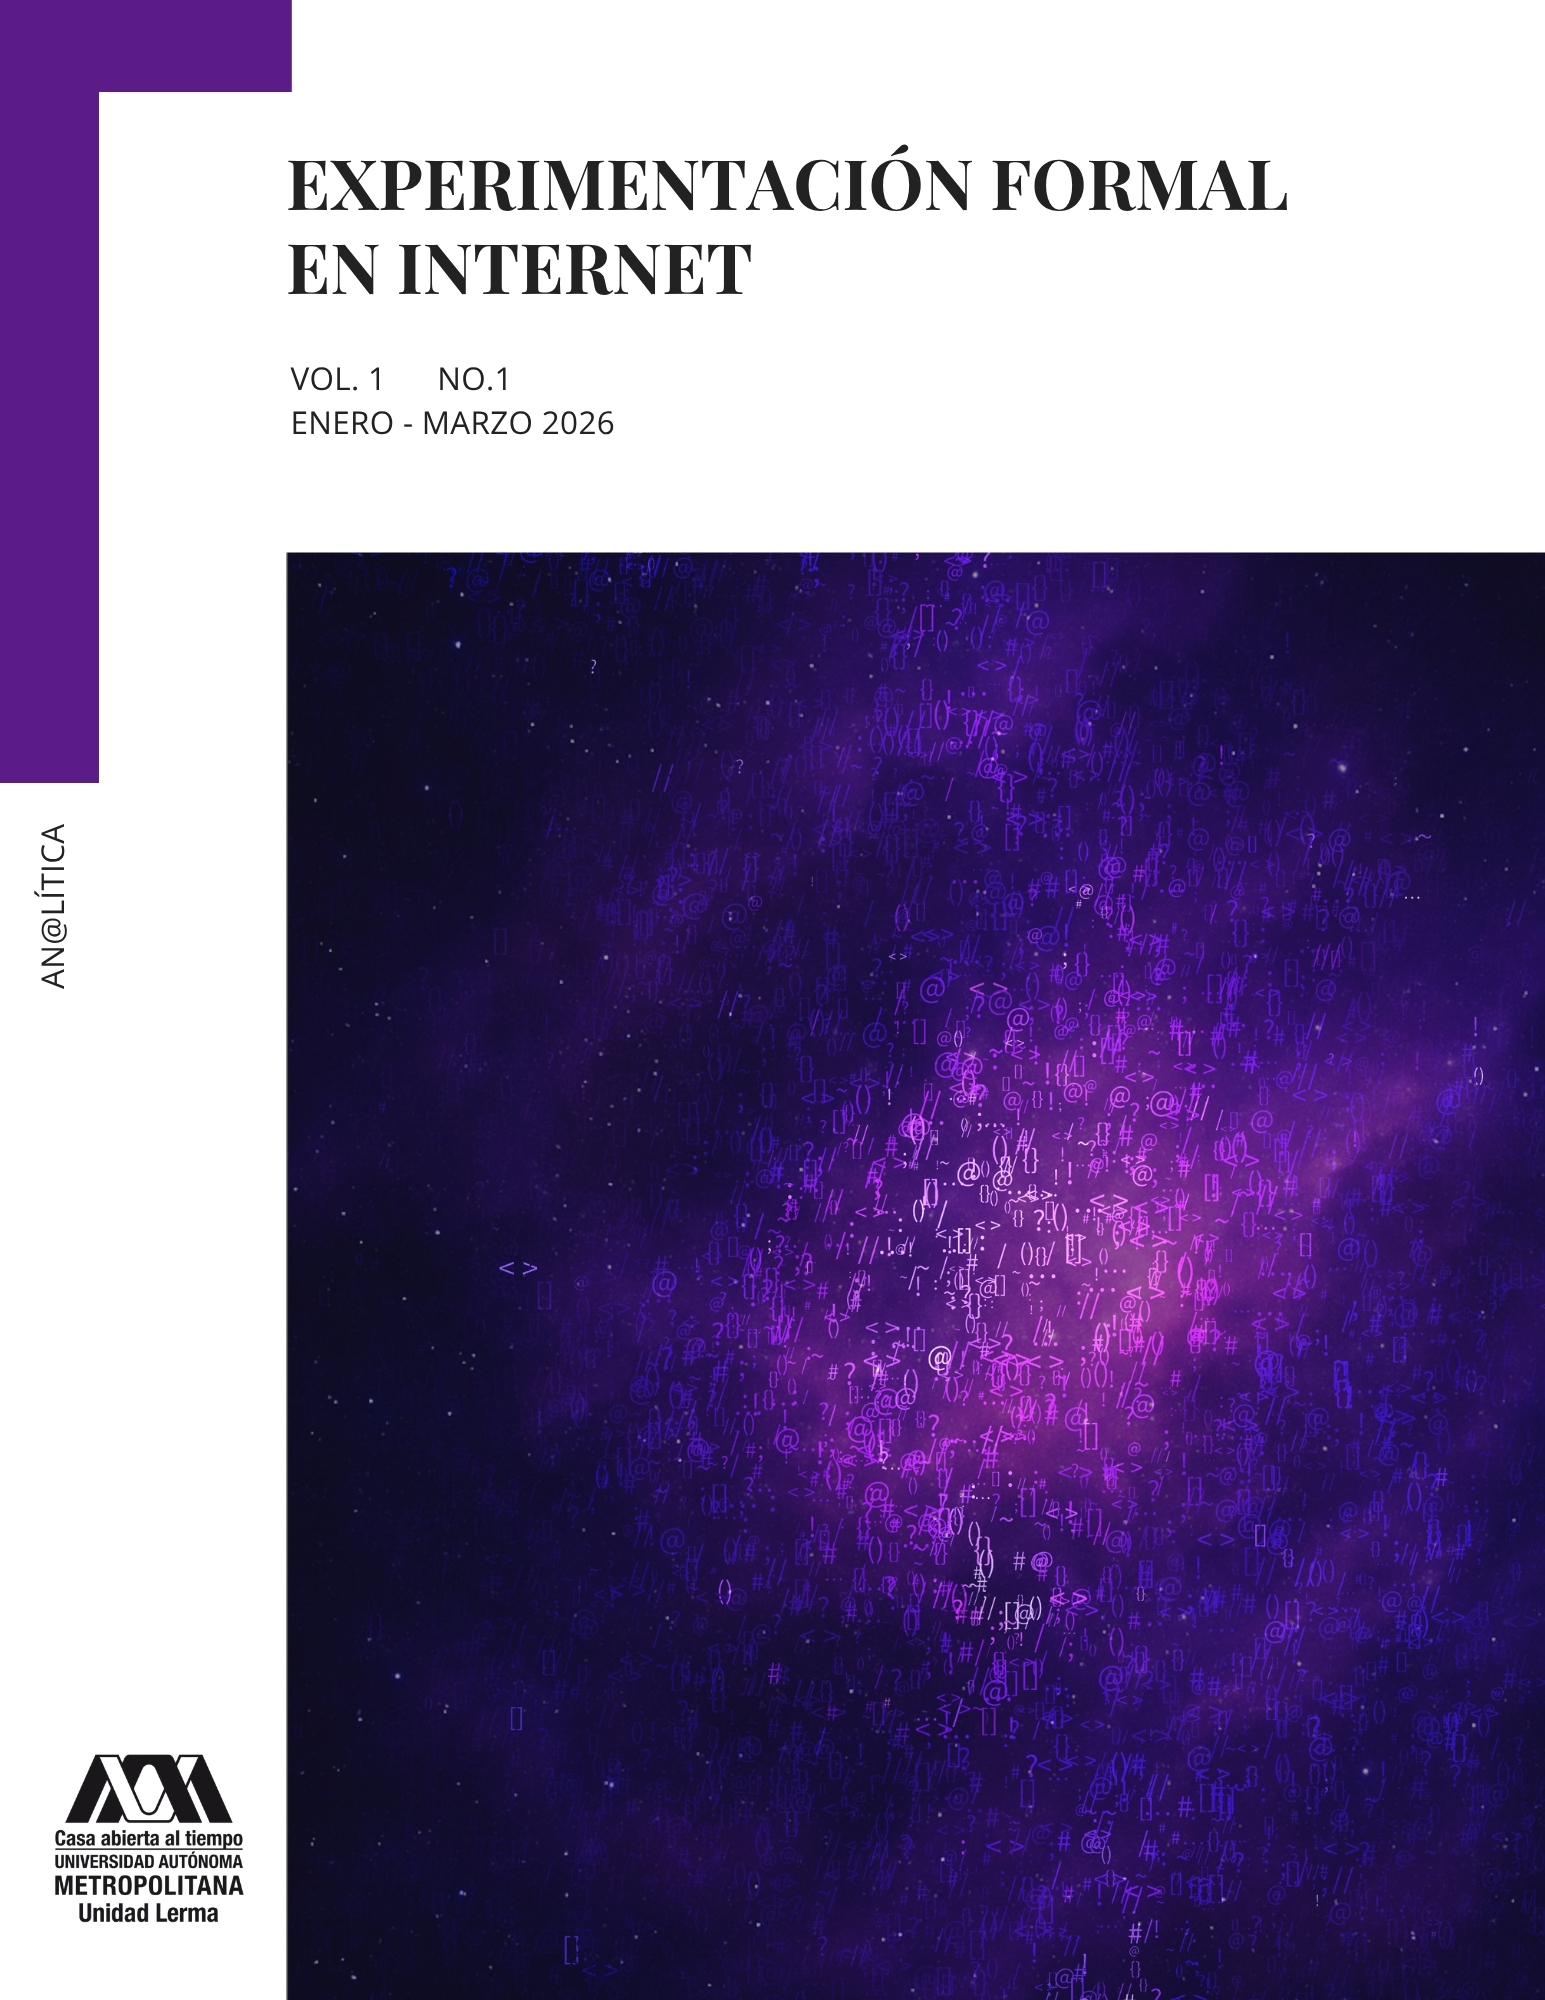
\includegraphics[width=1.1\textwidth]{assets/imagenes/portada.jpg}

\end{titlepage}

% ============================================
% PÁGINA 2: EN BLANCO
% ============================================
\clearpage
\thispagestyle{empty}
\pagestyle{empty}
\mbox{}  % Página vacía
\clearpage

% ============================================
% PÁGINA 3: CINTILLO (MEDIA PORTADA)
% ============================================
\clearpage
\thispagestyle{empty}
\pagestyle{empty}


\raggedright
    % TÍTULO (Negritas, tamaño grande)
    \LARGE \textbf{Políticas Públicas y Etnografía} \\

    \vspace{0.3cm}
    
    % SUBTÍTULO (Normal, más pequeño)
    \large Observando al Estado y como el Estado \\
    
    \vspace{1cm} % Espacio generoso entre título y autor (estilo Siglo XXI)
    
    % AUTOR (Tamaño grande, normal)
    \LARGE Abraham Zaíd Díaz Delgado \\
    
    \vspace{0.3cm}
    
    % ROL (Tamaño normal)
    \large Coordinador \\
    
% =========================================
% PÁGINA 3.1:IMÁGENES EN LA PARTE INFERIOR
% =========================================
    \vfill  % Empuja todo el contenido siguiente al fondo de la página
    \vspace{2.5cm}
    
    \begin{minipage}[t]{0.48\textwidth}  % 48% del ancho de texto
        
\includegraphics[width=1.5\textwidth]{../../institucionales/assets/logos/logo_uam_l.png}  % Imagen al 50% del minipage
    \end{minipage}% Se puede agregar otra minipage abajo si es necesario ingresar otro logotipo
    
\clearpage

% ============================================
% PÁGINA 4: DATOS LEGALES / CRÉDITOS
% ============================================
\begin{titlepage}
    \thispagestyle{empty}
    \pagestyle{empty}
    
    \vspace*{2cm}
    
    \begin{center}
        \textbf{Políticas Públicas y Etnografía} \\
        \textit{Observando al Estado y como el Estado} \\
        \vspace{0.5cm}
        
        \small
        Coordinador: Abraham Zaíd Díaz Delgado \\
        Universidad Autónoma Metropolitana \\
        Unidad Lerma \\
        División de Ciencias Sociales y Humanidades \\
        \vspace{1cm}
        
        \rule{0.6\textwidth}{0.4pt}
        \vspace{0.5cm}
        
        \small
        \textbf{Datos de catalogación} \\
        \vspace{0.3cm}
        Primera edición, 2026 \\
        Lerma de Villada, Estado de México \\
        \vspace{0.3cm}
        ISBN: 978-xxx-xxx-xxx-x \\
        D.R. © 2026, Universidad Autónoma Metropolitana \\
        Unidad Lerma \\
        Av. Hidalgo Poniente 46, Col. La Estación, \\
        Lerma de Villada, Estado de México, C.P. 52006 \\
        \vspace{0.3cm}
        Impreso y hecho en México \\
        \vspace{0.3cm}
        Queda prohibida la reproducción total o parcial \\
        sin autorización escrita del titular de los derechos
    \end{center}
\end{titlepage}

% ============================================
% REGRESAR A ESTILO NORMAL PARA EL ÍNDICE
% ============================================
\pagestyle{plain}
\setcounter{page}{1}  % Reinicia numeración para el índice

\renewcommand*\contentsname{Índice}
{
\setcounter{tocdepth}{1}
\tableofcontents
}

\mainmatter
\bookmarksetup{startatroot}

\chapter*{Introducción}\label{introducciuxf3n}
\addcontentsline{toc}{chapter}{Introducción}

\markboth{Introducción}{Introducción}

\textbf{Abraham Zaíd Díaz Delgado}\footnote{Esta investigación formó
  parte del proyecto nacional de investigación e incidencia ``Estrategia
  transdisciplinaria de investigación y resolución en la problemática de
  los residuos sólidos urbanos, aplicada en 6 ciudades mexicanas'' del
  CIESAS unidad Golfo; apoyado por el Consejo Nacional de Humanidades,
  Ciencias y Tecnologías (Conahcyt) en el marco de las actividades del
  Programa Nacional Estratégico (PRONACES) Agentes Tóxicos y Procesos
  Contaminantes. Número de proyecto 321379.}

\addtocontents{toc}{\protect\hspace{1.5em}Abraham Zaíd Díaz Delgado\par}

Las políticas públicas (PP) repercuten en nuestras vidas, pues suponen
el funcionamiento de los engranajes políticos que los Estados nacionales
ponen en marcha para dar solución a circunstancias identificadas como
problemáticas dentro del orden social vigente. No es casualidad que su
estudio se centre en comprender qué hacen los gobiernos para que la
maquinaria opere tal como lo hace, con sus fallas ineludibles y sus
puntos perfectibles. Asimismo, permiten reflexionar en profundidad sobre
las razones que dan origen al orden dispuesto de los engranajes de la
maquinaria gubernamental, cuestionándose ¿por qué las piezas se
encuentran en esa posición y no en otra?, ¿cómo debe resolverse
determinado problema?, ¿qué tuvo que suceder paquartora que una realidad
fuera reconocida como un problema que solo el Estado puede resolver? Y,
sobre todo, ¿por qué en muchas ocasiones no logra darle solución? De
este modo, continúan surgiendo interrogantes sobre los efectos que las
potenciales soluciones tienen en realidad, dado que las políticas
públicas son, en esencia, una compleja matriz de toma de decisiones
humanas guiadas por el imperativo ideológico que reivindica la
legitimidad del Estado y de sus instituciones. Bajo este enfoque,
resulta necesario indagar, en un nivel empírico, en la experiencia de
los diversos agentes que participan en el complejo entramado de fuerzas
políticas que conforman las políticas públicas.

Este libro titulado ``Políticas Públicas y Etnografía. Observado al
Estado y como el Estado'' tiene como objetivo adentrarse en los mundos
de significados autocontenidos en el universo de las políticas públicas
valorando la diversidad de voces, posiciones y experiencias en la
atención de problemáticas sociales particulares, por lo tanto, he de
advertir a los lectores que este no es un compilado de desarrollo
riguroso de los marcos teóricos hegemónicos en el estudio de las PP, más
bien encontrará un cúmulo de experiencias que, aunque distantes espacial
y temporalmente, coinciden con la necesidad de someter a debate las
implicaciones personales, afectivas y profesionales que interpelan a
diversos investigadores sociales en su vinculación con las PP.

Este libro tiene como propósito abrir un espacio para el debate
científico que recoja la reflexión crítica en torno a la experiencia de
quienes, en calidad de investigadores sociales, participan en alguna
fase del ciclo de las políticas públicas (PP). Esta perspectiva se funda
en el reconocimiento de un nivel de análisis que ha sido poco explorado
hasta la actualidad, cuya relevancia académica y operativa encierra un
potencial significativo que solo se revela plenamente cuando la práctica
se sostiene en el tiempo, se cuestiona y comparte para ser sometido a un
debate productivo. En este sentido, las experiencias etnográficas que
aquí se presentan constituyen fuentes valiosas para dar continuidad a un
aprendizaje colectivo, siendo capaces de atenuar la atomización de los
esfuerzos investigativos y de replantear la visión común que considera
los resultados del estudio de las PP como procesos distantes, fríos,
impersonales y estériles.

Los trabajos de investigación reunidos en este libro constituyen una
selección de material idóneo para la identificación de casos de
referencia que permitirán realizar estudios de política comparada, con
el agregado de que en ellos se ofrecen las descripciones densas
elaboradas por los autores que, en la mayoría de los casos, ocuparon
posiciones privilegiadas desde las cuales lograron reconocer tanto las
virtudes como las áreas de oportunidad en el abordaje de los problemas
sociales contemporáneos a través de políticas públicas específicas.

En el primer capítulo, Abraham Zaíd Díaz Delgado revisita
etnográficamente su experiencia profesional en la dependencia operadora
de la política de telecomunicaciones en México durante los años 2024 y
2025, mostrando que, en el seno de las políticas públicas (PP), se
debaten y definen distintas perspectivas de la idea hegemónica del
Estado, así como del discurso gubernamental de la llamada ``Cuarta
Transformación'' (4T), en este caso particular. Destaca que la política
de telecomunicaciones funge como punto de encuentro entre el desarrollo
tecnológico y la consolidación de un régimen político. En lo que toca a
los retos de la PP del sector, se reconoce la necesidad de superar la
contradicción entre el discurso de justicia social de la 4T y la
complejidad real que esta implica, así como el hecho de que la política
de telecomunicaciones es reflejo de dicha inconsistencia. Además, señala
que la superación de la brecha digital está atravesada por sesgos de
carácter técnico que no son necesariamente vinculantes con la
dignificación de los medios de vida de las poblaciones incomunicadas.
Otro aspecto que remarca este trabajo es que la brecha digital reproduce
brechas sociales de clase, lo que la convierte en un fenómeno
predominantemente político. Asimismo, el texto ilustra la coyuntura
política del cambio institucional en México con la llegada al poder del
partido MORENA, proceso que ha generado contradicciones y desaciertos en
la operación de las PP. Pero, principalmente, abre un panorama novedoso
sobre el potencial explicativo de la etnografía para el ciclo de las
políticas públicas, no solo como un método de extracción de información
para su diagnóstico, implementación y evaluación, sino también como una
herramienta aplicada a los mecanismos internos y a los andares
cotidianos que involucran a funcionarios públicos, operadores de las PP
y población beneficiaria, desde una lectura crítica de la antropología y
etnografía política, del Estado, la ley y las instituciones,
introduciendo una vía analítica no exenta de originalidad para las
ciencias sociales y la función pública.

En el segundo capítulo Marco Rodríguez y Nancy Jiménez analizan el
impacto de la política social del régimen de gobierno actual en México,
autodenominado de ``la cuarta transformación'' (4T), en los trabajadores
formales e informales del sector de residuos, específicamente en
Acapulco (Guerrero), Oaxaca de Juárez (Oaxaca), Tlaxcala (Tlaxcala) y
Cuetzalan (Puebla) con aquellos que cumplen las tareas de procesamiento,
recolección, traslado y tratamiento de desechos sólidos. El estudio
emplea un enfoque mixto que abona al diálogo entre la profundidad
descriptiva con visión panorámica de los datos estadísticos e
indicadores de evaluación a fin de proponer una alineación entre
políticas públicas a diversas escalas y niveles de gobierno. La
pertinencia de esta investigación radica en tomar como punto de partida
el perfil socioeconómico de los trabajadores resultando que, debido a la
condición marginal en la que suelen vivir, son objeto de múltiples
programas de asistencia social, en un principio, porque la cobertura de
manutención que otorga su remuneración como trabajadores del sector de
residuos es insuficiente. Aunado a ello, la aplicación a formar parte de
otros programas sociales acarrea una serie de obstáculos que deben
sortear y que recrudecen la condición de vulnerabilidad en la que están
sumergidas sus familias. Otra virtud del trabajo de los autores es
reconocer la desigualdad como una condición sine qua non para
determinadas políticas sociales y la recolección de datos en diversos
contextos dentro del territorio mexicano demuestra que fungen también
como mecanismos de diferenciación revitalizando diversas violencias,
sobre todo la económica, de manera estructural. Con todo, la corrección
que promueve el capítulo insta a alineamiento de multiescalar de la
política social para dignificar la vida de los sectores marginados y
puntualmente del sector laboral de la gestión de residuos sólidos.

El tercer capítulo autoría de Enver Vargas y David Alzate profundiza en
el análisis crítico de categorías dominantes que fundan las bases sobre
las cuales se diseña, implementa y evalúan las políticas públicas desde
la valoración de la subjetividad y reflexividad en la investigación,
dichas categorías se reflejan en la noción del Estado como ente unitario
o monolítico, la legitimidad en el actuar gubernamental y la
impersonalidad con que la burocracia asume a las personas,
objetivándolas y despojándolas en la práctica de su calidad de sujetos
de derecho cuando han de entrar en acción los fundamentos estatales para
su protección como lo son las políticas públicas. Los autores de origen
colombiano comparten las etnografías de dos casos concretos en su país
para ello; el primero de ellos aborda la operación del Programa de
Defensoría del Pueblo en un momento de emergencia humanitaria frente a
las violaciones de derechos humanos perpetradas en el contexto de los
años del conflicto armado por las guerrillas en aquel país y el segundo
expone una red criminal en el Departamento Administrativo de Seguridad
luego de encontrarse culpables a diversos funcionarios públicos que
colaboraron en el despliegue criminal en ese mismo contexto. Es
importante reconocer que ambos casos de estudio oscilan entre la
``técnica y la política'' a decir que los autores, dejando de manifiesto
una posición parcial y pragmática necesaria para poder desarrollar una
exploración etnográfica de mayor alcance y multivocal, esto es algo que
constantemente ha de hacerse en casos de corrupción y violencia como los
aquí atendidos. Por si fuera poco, hace presencia otro tipo de abordaje
etnográfico conocido como ``etnografía documental'' que somete a
cuestionamiento las estructuras que consolidan los archivos y documentos
que soportan los relatos comúnmente hegemónicos de un momento histórico,
por lo común, en entornos de riesgo y conflicto esta clase de etnografía
es de gran utilidad; siendo este capítulo un claro ejemplo. En suma,
Vargas y Alzate demuestran el borramiento y superación de las nociones
de típicamente evocan la idea de Estado, sus procesos y políticas
securitarias que, específicamente en Colombia se ven excedidos en la
atención del trauma emanado del conflicto armado y porque ese daño se
produjo, en parte, por el entrelazamiento entre estatalidad y
criminalidad.

El capítulo cuatro coescrito por Omar Becerra, Tzitzi Becerra y
Francisco Ayala se ocupa de analizar el estado vigente de las políticas
públicas orientadas a la preservación y promoción de los patrimonios
culturales del estado de Michoacán, México, alertando sobre la
parcialidad de éstas y la necesidad de estrechar la vinculación con las
comunidades por el desconocimiento de las necesidades culturales reales
de la población incluyendo factores de orden económico, social y
ambiental a las políticas públicas locales en torno al patrimonio
cultural michoacano, afinando así el proceso de éstas y evitando su
operación de manera aislada como mecanismo de gobierno. Además, se
expone desde una perspectiva histórica el proceso institucional y legal
que rige hasta el día de hoy el entorno político del patrimonio material
e inmaterial con el que cuenta Michoacán, lejos de centrarse en un
programa o bien cultural específico, los autores demuestran elementos
contextuales sobre los cuales la etnografía se presenta como una
alternativa viable para la mejora de las políticas públicas culturales,
de las instituciones que las construyen y ejecutan, así como de la
construcción discursiva de la riqueza cultural y patrimonial local.
Finalmente, este capítulo colectivo sugiere que el aumento del
financiamiento estatal para fortalecer las cadenas de valor existentes
en materia cultural y, sobre todo, destaca la necesidad de involucrar a
las comunidades objetivo en el establecimiento de una agenda cultural
para un correcto diagnóstico e implementación de las políticas públicas
culturales en Michoacán.

En el capítulo quinto Alejandro Agudo ilustra las complejidades que
alberga la construcción de conocimiento y toma de decisiones en las
posiciones de ``antropólogo activista'' y ``antropólogo consultor''
empleando dos ejemplos prácticos que contrastan las condiciones,
directrices y demandas de cada escenario, si bien ambos contextos son
distintos, en ellos coincide la etnografía como parte central de las
funciones desarrolladas por el antropólogo y dan pie a cuestionamientos
profundos sobre la posibilidad de conciliar entre el activismo y la
consultoría orientados a la atención de poblaciones vulnerables.
Asimismo, el autor advierte desde su experiencia acumulada que existen
algunos riesgos y condicionamientos interpretativos involucrados en
estos distintos entornos de aplicación y construcción del conocimiento,
siendo quizá el más claro, la tendencia a caer en polos opuestos de la
práctica etnográfica. Por un lado, señala que la adopción de una postura
moral denunciante útil para evidenciar los legítimos reclamos por
justicia de sectores marginados sistemáticamente puede llevar al punto
de imposibilitar la visualización de soluciones de los problemas que les
aquejan e incluso reforzando una visión parcial del origen de dichos
problemas, así como obstaculizar el entendimiento de las formas en cómo
funciona la realidad social más amplia, lo que derivaría un diagnóstico
sesgado y limitante de la vulnerabilidad referida. Por otra parte,
aborda empíricamente la incidencia de agendas políticas externas a las
instituciones, dependencias, organismos y demás instancias encargadas de
llevar a cabo proyectos de consultoría que tienen a como prioridad
idear, articular, promover y emprender soluciones a problemas puntuales
para determinados sectores, mismas que derivan en procedimientos y
tratamientos de información que tiende a homogenizar los resultados en
informes, recomendaciones o archivos que desdibujan la profundidad
reflexiva de la etnografía y que pocas veces se basan realmente en las
reflexiones derivadas de ésta, uno de los factores transversales a estas
agendas es el tiempo, puesto que la etnografía deviene necesariamente en
una honda reflexión que lleva tiempo procesar y expresar en los términos
adecuados para su aplicación en contextos donde potencialmente podría
incidir. Finalmente, este capítulo cumple con uno de los fines
esenciales de este libro al poner en debate las contradicciones y
tensiones éticas que se han definido típicamente unos espacios como
académicos y otros como aplicados casi exclusivamente.

Virginia Ramírez presenta en el sexto capítulo los efectos que ha tenido
el levantamiento del muro fronterizo de los Estados Unidos para marcar
la división con el territorio mexicano en una colonia marginal de
Tijuana (Baja California) generando la reconfiguración del paisaje
urbano a través del desalojo y despojo de viviendas para construir
vialidades que agilicen la movilidad en esa ciudad. El capítulo de la
antropóloga va más allá de las políticas públicas como medio de acción
de un estado nacional, ya que el contexto de la frontera norte de México
se ve influido por la actual crisis de movilidad humana a escala global,
siendo la ciudad referida en esta etnografía donde se da el flujo de
migrantes más numeroso de todo el mundo. La investigación se inscribe en
el contexto del programa federal ``Viaducto Elevado Tijuana'', un
megaproyecto de infraestructura emprendido por el Estado mexicano para
dar abasto a la movilidad de la zona y que no solo ha generado cambios
en la concepción del espacio público, sino que ha devenido en un punto
de quiebre de las historias de vida de los habitantes de la colonia
Libertad. El capítulo también muestra la yuxtaposición de políticas
públicas que no se encuentran alineadas dada la preeminencia de agendas
que obedecen a intereses políticos, factores económicos y a la gestión
de crisis que desplazan y criminalizan familias además de precarizar las
condiciones de vida locales. Este caso particular hace gala de la
influencia que el gobierno estadounidense ejerce directa o
indirectamente en la política pública nacional en temas migratorios,
profundizando la identidad de Tijuana como una ciudad de paso e indigno
para la residencia. Adicionalmente, refleja que la vida de los afectados
por la construcción del viaducto ya se encontraba atravesada por
distintas violencias, lo que posibilitó designarlos como objetos
descartables para el desarrollo del megaproyecto, la falta de
oportunidades es un problema de larga data en donde el trabajo de los
``polleros'' se hizo popular hasta el día de hoy en el que ha sido
cooptado por grupos delincuenciales por los que impera la violencia en
la zona y hace (en algunos casos) que el desalojo promovido desde el
gobierno resulte en una opción razonable para conservar la vida.
Metodológicamente este capítulo tiene la virtud de emplear la etnografía
como hoja de ruta para conciliar y resolver problemas operativos sobre
la marcha del proyecto del viaducto, buscando colocar en primer plano a
las personas desalojadas e interesándose por los dilemas inherentes al
cambio que el proyecto generó en sus vidas.

Por su parte, el séptimo capítulo escrito por Edgar Flores expone como
la relación entre las prácticas sociales que permiten a las personas
apropiarse e identificarse con el paisaje urbano pueden dar sentido al
emprendimiento de políticas públicas destinadas al mejoramiento de las
condiciones de vida de zonas periféricas de la Zona Metropolitana del
Valle de México, a partir de la observación de la cotidianidad en áreas
públicas de recreación y esparcimiento como parques, plazas públicas y
complejos deportivos en el municipio de Ixtapaluca, Estado de México.
Pese a que las reflexiones no van orientadas a un programa o política
pública locas concreta, el autor busca que con la apertura y
flexibilidad que permite la etnografía se pueda trazar un puente que
vincule la experiencia habitual del espacio urbano con la toma de
decisiones a distintos niveles y órdenes gubernamentales. Cabe destacar
que el esfuerzo investigativo del etnógrafo ha decantado por apelar a la
objetividad y neutralidad para hacer esto posible, y con ello paliar la
tensión entre la complejidad y reflexión profunda para atender al
pragmatismo que muchas veces se le atribuye a los ciclos de la política
pública, a bien de dialogar entre ambas perspectivas y aminorar el caos
que la descripción densa de las situaciones cotidianas en los espacios
recreativos y los procesos micropolíticos de la toma de decisiones
pueden atraer. El autor también destaca la capacidad de la antropología
urbana para contribuir en el diseño de espacios públicos que coadyuven
al bienestar de las poblaciones circundantes dado que los espacios
pueden ser comprendidos como procesos socioculturales y políticos en sí
mismos en los cuales están insertados múltiples actores rompiendo con la
dicotomía tradicional entre sociedad y Estado. Finalmente, a partir de
la observación flotante se relatan las necesidades y utilidad que las
personas hacen de estos entornos comunes valorando el trabajo
etnográfico (y en general académico) como un elemento necesario y
vinculante dentro de las políticas públicas del espacio público.

En el capítulo ocho Julio Rodríguez da cuenta de múltiples áreas de
oportunidad en la atención pública que se brinda a adultos mayores en
situación de calle, pese a contar con funcionarios que manifiestan
vocación de servicio, las condicionantes estructurales de los programas
de asistencia a este sector se ven entorpecidos por limitantes
burocráticas y por la falta de disposición de recursos adecuados y
suficientes para cubrir con suficiencia las necesidades de este sector.
El texto se enfoca en presentar un análisis del trabajo desarrollado en
dos instancias públicas: DIF e INAPAM dentro del municipio de Naucalpan
de Juárez (Estado de México). Recientemente, en el contexto mexicano se
han promovido diversos programas de política social dirigidos a
beneficiar a la población de la tercera edad a través de inventivos
económicos y provisión de servicios básicos, sin embargo, estos
esfuerzos han sido estériles para contrarrestar la vulnerabilidad de
este grupo de edad como advierte el autor, su lectura crítica de estas
políticas develan que hacen parte de las bases de fundan la desigualdad
y exclusión de manera estructural, por lo que insistir en la formulación
de ambientes propicios para vivir una vejez digna es una tarea
impostergable para el Estado mexicano y en ella habrán de considerarse
variables más allá de la materialidad, dado que el bienestar es una
noción volátil que está en función del contexto histórico. La situación
de calle en adultos mayores es una realidad comúnmente ignorada u
omitida en la prescripción de políticas públicas de asistencia social,
excluyendo aún más a esas personas de alternativas de vida digna; además
los programas sociales emblemáticos del régimen actual en el país
demandan la superación de filtros burocráticos que no contemplan esas
realidades menesterosas y que la poca flexibilidad en sus procesos de
incorporación imposibilitan la debida atención a los más desfavorecidos
perpetuando la exclusión extrema.

El capítulo nueve, escrito por Laura Matamala se distingue por ir a las
bases morales del bienestar entendido desde el ejercicio de la caridad y
el humanitarismo en un albergue para enfermos y una casa hogar para
niños, ambos ejemplos someten a debate el carácter político de las redes
interinstitucionales de beneficencia que se proponen paliar los
problemas que emergen en poblaciones vulnerables ante la imposibilidad
estatal de proveer la cobertura de sus necesidades básicas. La autora
echa mano de un prolongado recorrido por instituciones de cuidado con
fundamentos religiosos para articular una autoetnografía que desencadena
profundas reflexiones sobre el entrelazamiento real entre el Estado y la
Iglesia hasta nuestros días, así como las funciones que cubren y,
además, expone el desbordamiento de las categorías predominantes en el
estudio los activismos y las labores de asistencia humanitaria desde las
ciencias sociales y humanidades. El valor la autoetnografía que compone
este trabajo exhibe también una serie de dilemas éticos, morales y
prácticos en la dicotomía entre investigación y activismo, develando que
la toma de decisiones a niveles operativos y gubernamentales demanda
adherirse a una postura siempre perfectible, por ejemplo, con la
participación de las organizaciones que proveen servicios humanitarios
en redes o como depositario de donaciones que permiten su
funcionamiento, pero que sin embargo, no son sometidas a mecanismos
rigurosos de transparencia como lo harían agencias del sector público.
Con todo y que el trabajo no aborda de manera directa la relación de la
autora con un programa o plan de política pública el análisis de su
propia experiencia en los espacios de atención humanitaria evidencian
que, al igual que la política pública, las motivaciones e ideales suelen
establecerse en alusión a una población objetivo mucho más imaginada que
real que homogeniza y esencializa a los sujetos beneficiarios como
receptáculos de las acciones institucionales lo que reduce la visión y
descarta su potencial de agenciamiento que, sin embargo, existe y que
les hace emprender diversas estrategias en pro de maximizar los recursos
obtenidos bajo su condición de vulnerabilidad.

Finalmente, el Comité Editorial de la División de Ciencias Sociales y
Humanidades de la Universidad Autónoma Metropolitana, Unidad Lerma, y la
coordinación del libro ``Políticas Públicas y Etnografía. Observado al
Estado y como el Estado'' expresamos nuestro más profundo agradecimiento
a los autores que han nutrido este espacio con trabajos de investigación
de alta calidad y relevancia para nuestra actualidad. Asimismo,
reconocemos a los dictaminadores anónimos de cada contribución, quienes
participaron en el proceso de revisión por pares ciegos, procurando la
calidad académica de este número y compartiendo generosamente parte de
su tiempo y conocimiento de manera voluntaria. Finalmente, se invita a
los lectores a fomentar el debate alrededor de este nicho de
investigación emergente pero fecundo donde confluyen las tensiones,
paradojas y contradicciones propias de las políticas públicas y la
etnografía, las cuales merecen ser objeto de estudio y reflexión.

\bookmarksetup{startatroot}

\chapter{Los retos de la brecha digital en México. Reflexiones
etnográficas de la política de telecomunicaciones
2024-2025}\label{los-retos-de-la-brecha-digital-en-muxe9xico.-reflexiones-etnogruxe1ficas-de-la-poluxedtica-de-telecomunicaciones-2024-2025}

Abraham Zaíd Díaz Delgado

Cerrar la brecha digital requiere el análisis crítico de las condiciones
de vida de las poblaciones más marginadas del país, así como de la razón
gubernamental que determina las políticas públicas en materia de
telecomunicaciones. Este capítulo invita a descentrar las soluciones de
los aspectos técnicos y de infraestructura y a idear estrategias
integrales de orden sociocultural y político como lo pueden ser la
alfabetización tecnológica, el desarrollo institucional tanto a nivel
operativo como en la percepción dentro de la esfera pública y; que
fomenten la confianza en las TIC´s y en las telecomunicaciones como nodo
articulador de la gobernanza democrática.

\hfill\break

\section*{Intro}\label{intro}

\markright{Intro}

\addtocontents{toc}{\protect\hspace{1.5em}Abraham Zaíd Díaz Delgado\par}

Cerrar la brecha digital requiere el análisis crítico de las condiciones
de vida de las poblaciones más marginadas del país, así como de la razón
gubernamental que determina las políticas públicas en materia de
telecomunicaciones. Este capítulo invita a descentrar las soluciones de
los aspectos técnicos y de infraestructura y a idear estrategias
integrales de orden sociocultural y político como lo pueden ser la
alfabetización tecnológica, el desarrollo institucional tanto a nivel
operativo como en la percepción dentro de la esfera pública y; que
fomenten la confianza en las TIC´s y en las telecomunicaciones como nodo
articulador de la gobernanza democrática.

\bookmarksetup{startatroot}

\chapter{Condiciones de trabajo y acceso a programas sociales en el
sector de residuos: insumos para una política social en municipios de
México}\label{condiciones-de-trabajo-y-acceso-a-programas-sociales-en-el-sector-de-residuos-insumos-para-una-poluxedtica-social-en-municipios-de-muxe9xico}

Marco Antonio Rodríguez Gómez y Nancy Merary Jiménez Martínez

Este trabajo examina si la política social de la cuarta transformación
beneficia directa o indirectamente a la población trabajadora del sector
de residuos sólidos en tres ciudades medias y un municipio rural en
México. A partir de un análisis mixto sobre sus condiciones
socioeconómicas y la cobertura de los programas sociales que más los
favorecen, se encontró que, aunque algunas personas trabajadoras y sus
familias reciben beneficios indirectos, la cobertura directa es limitada
y persisten barreras de acceso. El artículo concluye que la oferta
universal de programas sociales no revierte la vulnerabilidad social de
este sector, por lo que propone una orientación focalizada como
complemento redistributivo para interrumpir el ciclo de pobreza y
precariedad que enfrentan.

\hfill\break

\section*{Intro}\label{intro-1}

\markright{Intro}

\addtocontents{toc}{\protect\hspace{1.5em}Marco Antonio Rodríguez Gómez y Nancy Merary Jiménez Martínez\par}

\bookmarksetup{startatroot}

\chapter{Introducción}\label{introducciuxf3n-1}

El objetivo de este artículo fue desarrollar un análisis y propuesta de
alineación de los programas sociales federales hacia la población que
trabaja de manera formal e informal en los sistemas de gestión de
residuos sólidos urbanos en las ciudades de Acapulco, Oaxaca y Tlaxcala,
todas capitales de sus estados, así como el municipio de Cuetzalan, que
tiene un carácter rural e indígena\footnote{Esta investigación formó
  parte del proyecto nacional de investigación e incidencia ``Estrategia
  transdisciplinaria de investigación y resolución en la problemática de
  los residuos sólidos urbanos, aplicada en 6 ciudades mexicanas'' del
  CIESAS unidad Golfo; apoyado por el Consejo Nacional de Humanidades,
  Ciencias y Tecnologías (Conahcyt) en el marco de las actividades del
  Programa Nacional Estratégico (PRONACES) Agentes Tóxicos y Procesos
  Contaminantes. Número de proyecto 321379.}.

Aunque Acapulco (Guerrero), Oaxaca de Juárez (Oaxaca), Tlaxcala
(Tlaxcala) y Cuetzalan del Progreso (Puebla) no conforman una región
geográfica o administrativa unificada, su inclusión en este estudio se
sustenta en un enfoque comparativo que busca capturar la diversidad
territorial y sociolaboral del personal empleado en el sector de los
residuos en México. Estos municipios representan distintos tipos de
contexto ---urbano turístico, ciudad patrimonial, intermedio-industrial
y rural-indígena--- que permiten analizar si la precariedad laboral se
configura en función del tipo de territorio y su estructura
socioeconómica.

Este análisis abarcó dos aspectos importantes: un diagnóstico detallado
de las condiciones sociodemográficas y laborales de la población
trabajadora formal e informal y de la cobertura de los programas
sociales federales que recibe este grupo laboral y sus familias. Para
lograrlo, se levantó información de primera mano y se hizo un análisis
documental de los principales programas sociales federales que los
benefician. A partir de lo anterior, se propone una alineación de estos
instrumentos de política social hacia esta población, fin de garantizar
su cobertura y atención de sus necesidades más urgentes, lo cual sienta
las bases para el diseño de estructuras que abonen a la construcción de
una Economía Circular Solidaria y Social en nuestro país.

El artículo se organiza de la siguiente manera: se presenta el
diagnóstico del problema y se propone un encuadre conceptual para
abordarlo, posteriormente se expone el marco metodológico del trabajo y
la parte final se dedica a la presentación de resultados, su discusión y
las conclusiones de esta investigación.

\bookmarksetup{startatroot}

\chapter{Diagnóstico del Problema}\label{diagnuxf3stico-del-problema}

México, al igual que otros países, ha adoptado políticas neoliberales
que han reconfigurado la estructura institucional del país. Estas
políticas, caracterizadas por la acumulación de capital mediante la
flexibilidad laboral y la reducción de beneficios para la fuerza de
trabajo (Harvey, 2007), han generado un panorama marcado por el
incremento de la población con bajos ingresos y escasa cobertura de
seguridad social (Martı́nez, Marroquı́n, y Rı́os, 2019). En este contexto,
una proporción significativa de la fuerza laboral ha sido empujada hacia
la informalidad laboral, entendida como cualquier actividad laboral que
no está regulada ni tiene la protección del Estado (Hart, 1971). En esta
línea, Sassen (1991) exploró cómo la globalización y la reestructuración
económica influyen en el crecimiento del sector informal, especialmente
en las grandes ciudades del mundo, y encontró que la economía informal
es una respuesta a las nuevas formas de organización del trabajo
impuestas por la globalización. Esta dinámica es particularmente
evidente en el sector de los residuos sólidos urbanos, donde las
personas trabajadoras formales como informales se encuentran expuestas a
estas transformaciones estructurales que impactan negativamente su
calidad de vida.

En el ámbito formal, las personas trabajadoras suelen estar vinculadas a
sistemas municipales o empresas concesionarias que operan bajo un marco
legal. Sin embargo, Espinosa (2013) advierte que estas regulaciones no
garantizan condiciones laborales dignas. A pesar de contar con un empleo
público, enfrentan contratos inestables, ingresos insuficientes y
carencia de equipos de protección personal. Sin embargo, esta situación
no es exclusiva de México, en América Latina, Acurio, Rossin, Teixeira,
y Zepeda (1997) encontraron que la población trabajadora formal del
sector rara vez acceden a prestaciones laborales plenas, lo que la sitúa
en desventaja económica y social; pero al comparar las condiciones de
esta población laboral mexicana con aquella de ciudades como Sao Paulo o
Buenos Aires, Villanova (2012) señala que los ingresos de los
connacionales son más bajos, lo que exacerba su vulnerabilidad.

Por otro lado, el sector informal de residuos, conformado por personas
recolectoras independientes y recuperadoras de base, opera al margen de
una relación contractual y corresponde a una estrategia de sobrevivencia
en respuesta a la pobreza urbana Tevera (1993). El Programa de las
Naciones Unidas para el Medio Ambiente (2018) apunta que una
característica común en los países de América Latina es la presencia de
estas personas trabajadoras, a quienes considera consecuencia de las
crisis económicas y políticas habituales en la región que arrojan a un
sinnúmero de personas a la pobreza. Por ejemplo, en Argentina, Perelman
y Boy (2010) identificaron cómo las crisis económicas de principios de
los años 2000 llevaron un número significativo de personas a dedicarse a
la recuperación de residuos en las calles como alternativa para su
supervivencia.

Y aunque desempeñan un papel crucial en la recuperación de residuos
valorizables, el trabajo de estas personas carece de reconocimiento
formal, lo que se traduce en la ausencia de derechos laborales, acceso a
servicios de salud o vivienda y protección social (Espinosa, 2013).
Valente, Castillo, y Guevara (2019) incluso destacan que los gobiernos
municipales aprovechan frecuentemente la labor de estas personas sin
reconocer su contribución, perpetuando su precarización. Quienes, además
enfrentan condiciones insalubres, estigmatización social y la amenaza de
desplazamiento por iniciativas de formalización que no consideran sus
necesidades específicas (Favela, Ojeda, Cruz, Taboada, y Aguilar,
2013)\footnote{En este trabajo se consideraron trabajadoras informales a
  las personas que por cuenta propia recorren las calles a pie, previo
  al paso del camión recolector y se dedican a la pepena o recuperación
  de materiales depositados en las bolsas de basura para venderlos y
  obtener un ingreso; así como a las personas que, con el mismo fin,
  extraen residuos valorizables en estaciones de transferencia o sitios
  de disposición final.}. En suma, el personal laboral formal e informal
del sector de los residuos comparte problemas estructurales que limitan
su desarrollo vital. Entre estas problemáticas se encuentran la
inestabilidad en el empleo, bajos salarios, falta de protección social y
jornadas laborales prolongadas. Pero también, se le puede señalar como
parte de grupos sociales o minorías marginadas y sin escolaridad
(Besiou, Georgiadis, y Van Wassenhove, 2011). Estas condiciones reflejan
una precarización generalizada en el sector de los residuos, lo que les
impide ejercer plenamente su ciudadanía económica, política y social.

Este escenario cobra relevancia en un contexto donde la política social
de la Cuarta Transformación, diseñada bajo principios de universalidad,
busca garantizar el acceso a programas sociales sin condicionamientos
previos (Gobierno de México, 2019). A pesar de los principios de
universalidad, la cobertura de los programas sociales federales no ha
sido analizada en su capacidad para incluir al personal laboral formal e
informal del sector residuos; es decir, para dilucidar qué tanto esa
universalidad les acerca los beneficios de la política social y en todo
caso, avizorar de qué forma podría orientarse a su favor.

\bookmarksetup{startatroot}

\chapter{Encuadre conceptual}\label{encuadre-conceptual}

Las reformas de corte neoliberal implementadas en México han
transformado la estructura institucional del Estado, afectando múltiples
ámbitos sociales, económicos y laborales. Estas transformaciones
incluyen procesos como la descentralización administrativa, la
privatización de empresas paraestatales, la apertura de mercados
internacionales y la flexibilización laboral. Harvey (2007) identifica a
la flexibilización como un eje central en este modelo, subrayando su
impacto en la precarización del empleo: reducción de salarios, pérdida
de beneficios laborales y aumento de la inseguridad laboral.

La flexibilización del empleo ha implicado una reducción de los derechos
laborales, como la contratación colectiva, la estabilidad contractual y
las prestaciones. Esta transformación ha dado lugar a distintas
expresiones de la precarización laboral, entendidas como condiciones que
profundizan la vulnerabilidad socioeconómica del personal asalariado.
Rubio (2017) señala que la precariedad se expresa en la degradación de
las condiciones y relaciones de trabajo, repercutiendo en la
temporalidad, la insuficiencia salarial, la exposición a ambientes
laborales inseguros y la ausencia de protección social. Por su parte,
Lorey (2016) sostiene que la precariedad no se limita al ámbito
contractual, sino que opera como una forma de vulnerabilidad de lo
viviente, gestionada como dispositivo social de distribución del riesgo
mediante el control político de la vulnerabilidad vital (en el
neoliberalismo). En este marco, la precarización se expresa en el
deterioro de las condiciones laborales como en los procesos de
segmentación y subordinación de la vitalidad social de este personal
ocupado.

Por otro lado, la informalidad laboral ha emergido como vía de inserción
para sectores de la población ante una progresiva degradación del
trabajo asalariado. La consolidación del sector informal responde a
condiciones institucionales que involucran marcos legales y
racionalidades empresariales (Loayza y Sugawara, 2009). Aunque admite
múltiples interpretaciones, este encuadre se centra en sus implicaciones
sobre la provisión de prestaciones y remuneraciones legales, y en su
impacto directo sobre la calidad de vida.

En este sentido, Tokman (2001) interpreta la informalidad como una
estrategia de subsistencia frente a la escasez de empleos de calidad. No
obstante, Marinescu y Bratiloveanu (2020) proponen que la vinculación al
trabajo informal puede responder a una decisión individual,
especialmente cuando las diferencias entre empleo formal e informal se
perciben como mínimas. Diversos estudios señalan que la inserción
informal se distribuye de manera desigual entre grupos sociales: afecta
con mayor intensidad a mujeres (Sánchez, Robles, y Vargas, 2022),
personas casadas (Huesca y Padilla, 2012), jóvenes no cualificados o
personas adultas mayores (Marinescu y Bratiloveanu, 2020), migrantes con
bajos niveles de escolaridad (Lara, Cruz, Moyeda, Prats, y Téllez,
2020). Asimismo, (López, 2017) advierte que esta condición laboral
limita el acceso a la protección social, servicios fundamentales como
vivienda, salud, pensión. En consecuencia, la informalidad no solo
emerge como respuesta ante la precarización del empleo asalariado, sino
como régimen de inserción que restringe el ejercicio efectivo de la
ciudadanía económica y condiciona las trayectorias vitales de quienes
dependen de ingresos irregulares y desprotegidos.

En este escenario, la precarización y la informalidad pueden entenderse
como dos dimensiones complementarias de un mismo proceso de
transformación del mercado de trabajo. Ambas configuran un patrón
laboral marcado por la desregulación, la discontinuidad del trabajo y el
debilitamiento de los derechos socioeconómicos, lo que configura a la
fuerza de trabajo como población potencialmente vulnerable y expuesta a
la exclusión social. Tal como plantea Rizo (2006), la exclusión se
manifiesta como una acumulación de rupturas sucesivas en los ámbitos
económicos, político y social, donde el trabajo deja de ser un vehículo
de integración y pasa a representar un eje de desigualdad estructural.
En este sentido, la exclusión afecta la reproducción material del
individuo y su familia y erosiona la calidad de ciudadanía, minando su
acceso efectivo a derechos sociales básicos.

Es aquí donde la política social adquiere relevancia como instrumento
compensatorio (Cohen y Franco, 2005), orientado no sólo a la
transferencia de recursos, sino a la reconstitución de los vínculos de
integración que la exclusión social fractura. El Estado enfrenta el reto
de garantizar condiciones mínimas de inclusión que habiliten el
ejercicio pleno de ciudadanía. Siendo lo anterior una manera de mirar,
se despliega un campo de intervenciones sociales estatales centradas en
las condiciones de vida y de reproducción de la vida de la población
(Danani, 2017). Así, la política social se distingue por tener como
objeto la vida social y la vida de los sujetos, en tanto reproducción o
modelado de procesos y relaciones de vida de distintos grupos y clases
sociales.

Sin embargo, las intervenciones sociales del Estado no operan en un
vacío institucional. Su despliegue se inserta en una estructura social
que organiza de manera desigual el acceso a derechos, recursos y
condiciones de vida. Para comprender esta configuración, resulta
pertinente el enfoque estructural de Adelantado, Noguera, Rambla, y Sáez
(1998), que permite analizar cómo la política social no solo responde a
las desigualdades existentes, sino que también puede contribuir a su
reproducción o transformación, según los principios y dispositivos que
la orienten.

La estructura social se concibe como ``la configuración de
instituciones, reglas y recursos que asignan condiciones de vida
desiguales a las personas en un tiempo y lugar determinados''
(Adelantado et al., 1998). Esta concepción reconoce cuatro esferas
analíticas que constituyen la estructura social: mercantil, estatal,
doméstico-familiar y relacional. En el contexto de este análisis, las
esferas estatal y doméstico-familiar adquieren especial relevancia. En
la primera se concentran las capacidades regulatorias del Estado y su
aparato administrativo en la distribución de bienes materiales o
simbólicos; en la segunda las relaciones de parentesco y cuidado que
sostienen la reproducción de la fuerza de trabajo. Ambas esferas
constituyen terrenos clave de transformación para la política social, ya
sea mediante la provisión de servicios o mediante la reproducción
social.

Las posiciones que ocupan las personas en la estructura social están
atravesadas por tres ejes propuestos por los autores: la condición
ciudadanía (acceso a los derechos jurídicos-políticos), la relación
frente al aparato estatal (usuarios, empleados o beneficiarios de
servicios sociales) y las capacidades asociativas (posibilidad de
organización y demanda colectiva). Estos ejes permiten analizar cómo
ciertas poblaciones, como el personal ocupado del sector de los
residuos, enfrenta obstáculos estructurales para ejercer plenamente sus
derechos sociales. También permite identificar los beneficios a los
cuales acceden ---o no--- mediante la política social.

Aunque el enfoque de Adelantado et al. (1998) permite comprender cómo la
política social se inserta en una estructura social diferenciada por
esferas y ejes de desigualdad, resulta necesario articular esta lectura
con los debates sobre el diseño institucional de los programas sociales
en América Latina. En contextos donde persisten modelos de universalismo
o focalización (Cohen y Franco, 2005), aproximaciones que integren ambas
perspectivas no debilitan la universalidad de derechos, sino que aspiran
a fortalecerla desde la heterogeneidad. En este marco, indagar si los
programas de política social universal impulsados durante la Cuarta
Transformación benefician a quienes trabajan en el sector de residuos
resulta clave para examinar su inclusión en función de las condiciones
particulares de vulnerabilidad que enfrenta.

\bookmarksetup{startatroot}

\chapter{Metodología}\label{metodologuxeda}

Se adoptó un diseño metodológico mixto que combinó métodos cuantitativos
y cualitativos, permitiendo una comprensión integral de las
problemáticas que enfrentan las personas trabajadoras de los sistemas de
gestión de los residuos sólidos urbanos en su acceso a los programas
sociales federales. Este enfoque facilita la integración de datos
numéricos con información contextual, enriqueciendo el análisis al
combinar perspectivas complementarias (Creswell y Creswell, 2014).

Para el acercamiento cuantitativo se diseñaron dos encuestas, una
dirigida al personal formal y otra para el personal informal. La primera
comprendió 62 reactivos y se dividió en siete secciones: datos
generales, estado de salud, aspectos laborales, aspectos económicos,
organización gremial, vivienda y acceso a programas sociales. La segunda
encuesta para el personal informal se conformó por 49 reactivos
divididos en siete secciones: datos generales, estado de salud, aspectos
laborales, material y venta, organización gremial, vivienda y acceso a
programas sociales.

El estudio tuvo un muestreo no probabilístico por conveniencia
(Hernández, 2021). Esto significa que la elección de las personas
trabajadoras no dependió de la probabilidad, sino de causas relacionadas
con las características de la investigación o los propósitos del
investigador (Hernández Sampieri, Fernández Collado, y Baptista Lucio,
2014), en este caso su condición de formalidad e informalidad y la
ubicación en los municipios de Acapulco, Oaxaca, Tlaxcala y Cuetzalan.
Sin embargo, se tuvo una expectativa de participación mínima deseada en
cada municipio, que buscó obtener 20 encuestas del personal formal y 20
del informal, este número obedeció a los recursos limitados de tiempo y
financiamiento para esta investigación y representaba el máximo
operativo posible que el equipo de trabajo podía abordar en campo,
considerando las dificultades logísticas, la dispersión territorial, la
informalidad del sector y las restricciones institucionales para acceder
a ciertos espacios laborales. No obstante, esto no se cumplió
completamente.

En el caso del personal formal se alcanzó la cuota en las ciudades de
Oaxaca (22 encuestas) y Tlaxcala (22 encuestas); en Cuetzalan, se
levantaron 18 encuestas, lo que correspondió al 100\% de trabajadores
del sector de los residuos; en Acapulco se levantaron 9 encuestas debido
a que el periodo del levantamiento de datos coincidió con la celebración
de varios eventos políticos que mantenían ocupado al personal, la
particularidad de la organización de sus cuadrillas de trabajo en esa
ciudad hizo que únicamente se pudiera encuestar a una cuadrilla de
personas.

El cumplimiento de las cuotas de participación del personal informal se
obstaculizó debido a temas de seguridad, pues muchos se encuentran en
situación de calle, migración y delincuencia organizada en las ciudades
de Acapulco, Oaxaca y Tlaxcala, donde se levantaron tres, seis y dos
encuestas respectivamente. En Cuetzalan, antes del cierre del sitio de
transferencia (en 2022 y 2023), se identificó la presencia de personas
trabajadoras informales; sin embargo, después del cierre se prohibió
esta actividad y estas personas se desplazaron a otras localidades, por
lo que no se levantaron datos en esa ciudad. En cambio, se consiguió
encuestar al personal informal que labora en el sitio de disposición
final ``Las Matas'' en Minatitlán, donde se levantaron 10 encuestas.

El levantamiento de datos se llevó a cabo entre abril y agosto de 2024.
Un equipo de tres personas realizó las encuestas de manera presencial e
\emph{in situ}. En el caso del personal formal, se solicitó autorización
a las direcciones de servicios públicos municipales de los municipios
mencionados. Para el personal informal, se acudió a informantes clave
para su ubicación y establecer confianza, quienes suelen ser de difícil
acceso debido a la naturaleza móvil de su ocupación y a que en muchas
ciudades esta actividad está prohibida. Durante el trabajo de campo se
atendieron las consideraciones éticas necesarias: las personas
participantes fueron informadas sobre los objetivos de la investigación
antes de participar y se garantizó su confidencialidad y anonimato.

Para la captura de datos se diseñaron dos formularios en Google Forms
donde se sistematizaron los datos, que después se exportaron a una hoja
de cálculo para su limpieza y organización. Posteriormente, se
procesaron los datos en Excel y se analizaron los estadísticos
descriptivos básicos.

Además, para la componente cualitativa del estudio se analizaron los
programas sociales federales mediante un trabajo de gabinete basado en
la revisión de documentos oficiales y evaluaciones de política pública.
Este método fue seleccionado porque proporciona una base normativa y
administrativa desde la cual contrastar la experiencia reportada por el
personal laboral con los objetivos declarados de los programas.

En primer lugar, se seleccionaron los programas relevantes a partir del
Plan Nacional de Desarrollo 2019-2024 (Gobierno de México, 2019), los
programas sectoriales y las reglas de operación priorizando aquellos
dirigidos a personas adultas mayores, personas con discapacidad
permanente y madres trabajadoras sin acceso a seguridad social.
Posteriormente, se analizaron los Diagnósticos para los Programas de
Nueva Creación para identificar los objetivos, la definición de
problemas, las causas estructurales y los efectos asociados que cada
programa busca atender. Esta información fue organizada en categorías
clave: programa, problemática atendida, causas, efectos y población
potencial y objetivo, asegurando una sistematización coherente y clara
para analizarlos a la luz de las encuestas aplicadas.

\bookmarksetup{startatroot}

\chapter{Resultados}\label{resultados}

En esta sección se presentan en primer lugar, los aspectos
sociodemográficos, escolaridad, distribución laboral y antigüedad, así
como jornadas laborales y contratación de las personas formales e
informales participantes. Posteriormente, se muestra cuáles son los
programas sociales federales que los benefician directamente y la
cobertura de estos en sus familias. Por último, se describen las
problemáticas que atienden los programas sociales federales, sus causas
y efectos, así como su cobertura y cómo se relacionan con los aspectos
sociodemográficos de los trabajadores del sector residuos cuando señalan
que son beneficiarios directos o indirectos.

De acuerdo con el Censo Nacional de Gobiernos Municipales y
Demarcaciones Territoriales de la Ciudad de México 2023, de los 2539
municipios que prestan el servicio de gestión de residuos sólidos
urbanos en México, en 89.7\% de los municipios el servicio es ofrecido
directamente por el ayuntamiento; en 7.6\% es privado; y en 2.6\% es
social. El personal laboral del sector se integra por 98,410 personas:
2.4\% en puestos de gerenciales y directivos, 4.4\% en posiciones
administrativas y contables y 93.2\% adscritas como personal técnico y
operativo; 86\% son hombres y 14\% son mujeres. Según su régimen de
contratación 49\% es de base o sindicalizada, 25\% de confianza, 16\%
eventual, 2\% por honorarios y 8\% tiene otro régimen de contratación
(INEGI, 2023). Estos datos apuntan que incluso entre el personal formal
hay una precarización laboral, ya que, aunque la mayoría labora para los
ayuntamientos, prácticamente la mitad del personal ocupado formal
experimenta degradación en sus condiciones y relaciones laborales,
caracterizadas por formas de contratación poco estables, temporales y
con ausencia de protección social.

En ese orden, los resultados de esta investigación dan cuenta que, en
cuanto a la distribución por género, el personal ocupado formal está
compuesto principalmente por varones (72\%), mientras que en el informal
la proporción masculina aumenta a 76\%. Las edades promedio son
similares en ambos grupos: 41.8 años para el formal y 41.7 años para el
informal; es decir, se trata de personas trabajadoras con trayectorias
laborales maduras, quizá con experiencia organizativa, además, se
esperaría que tuvieran cierta estabilidad laboral y una acumulación y
reconocimiento de sus derechos.

Por su situación familiar, se destaca que 68\% del personal formal y
58\% del informal se encuentran unidos (casados o en unión libre).
Además, el promedio de dependientes económicos es mayor entre las
personas trabajadoras formales (2.1) frente a las informales (0.9). Cabe
destacar que el número de dependientes es mayor en los trabajadores
formales varones (2.9) y en las trabajadoras informales (1.75)
respectivamente.

Las personas ocupadas del sector de los residuos, formales e informales,
comparten un porcentaje similar de analfabetismo (10\%). No obstante, el
rezago educativo es más evidente entre el personal informal: 43\% sólo
cuenta con estudios de primaria, en comparación con 14\% del personal
formal. La diferencia también se acentúa en los niveles superiores, ya
que 9\% del personal formal tiene licenciatura o posgrado, frente a sólo
5\% del informal (cuadro 1).

\begingroup
\scriptsize

\begin{longtable}[]{@{}
  >{\raggedright\arraybackslash}p{(\linewidth - 8\tabcolsep) * \real{0.2000}}
  >{\raggedright\arraybackslash}p{(\linewidth - 8\tabcolsep) * \real{0.2000}}
  >{\raggedright\arraybackslash}p{(\linewidth - 8\tabcolsep) * \real{0.2000}}
  >{\raggedright\arraybackslash}p{(\linewidth - 8\tabcolsep) * \real{0.2000}}
  >{\raggedright\arraybackslash}p{(\linewidth - 8\tabcolsep) * \real{0.2000}}@{}}
\caption{Escolaridad por nivel educativo y género. Elaboración
propia.}\label{tbl-1}\tabularnewline
\toprule\noalign{}
\begin{minipage}[b]{\linewidth}\raggedright
Escolaridad
\end{minipage} & \begin{minipage}[b]{\linewidth}\raggedright
Formales hombres (\%)
\end{minipage} & \begin{minipage}[b]{\linewidth}\raggedright
Formales mujeres (\%)
\end{minipage} & \begin{minipage}[b]{\linewidth}\raggedright
Informales hombres (\%)
\end{minipage} & \begin{minipage}[b]{\linewidth}\raggedright
Informales mujeres (\%)
\end{minipage} \\
\midrule\noalign{}
\endfirsthead
\toprule\noalign{}
\begin{minipage}[b]{\linewidth}\raggedright
Escolaridad
\end{minipage} & \begin{minipage}[b]{\linewidth}\raggedright
Formales hombres (\%)
\end{minipage} & \begin{minipage}[b]{\linewidth}\raggedright
Formales mujeres (\%)
\end{minipage} & \begin{minipage}[b]{\linewidth}\raggedright
Informales hombres (\%)
\end{minipage} & \begin{minipage}[b]{\linewidth}\raggedright
Informales mujeres (\%)
\end{minipage} \\
\midrule\noalign{}
\endhead
\bottomrule\noalign{}
\endlastfoot
Analfabetismo & 6 & 15 & 6 & 20 \\
Primaria & 14 & 15 & 44 & 40 \\
Secundaria & 32 & 60 & 31 & 20 \\
Preparatoria & 43 & 15 & 13 & 20 \\
Licenciatura o superior & 9 & 10 & 5 & 0 \\
\end{longtable}

\endgroup

Entre las personas trabajadoras formales, la antigüedad promedio en el
empleo es de 7.5 años, con un rango de entre tres meses y 35 años. En
este grupo, todas las personas encuestadas declararon trabajar para el
ayuntamiento (49\% en el área de barrido, 8\% como choferes de camión,
8\% en recolección, 8\% supervisión, 8\% como suplentes, 10\% en otro
tipo de trabajo). Por su parte, las personas trabajadoras informales
tienen una antigüedad promedio de 11 años, con un rango de seis meses a
42 años. Esto significa que tienen más tiempo en el oficio que quienes
trabajan en los sistemas formales y que una vez que ``entran'', hacen de
esta actividad su empleo para toda la vida. Esto coincide con lo
encontrado en otro estudio sobre recuperadores y recuperadoras de
residuos (Jiménez y De Castro, 2019; Tevera, 1993).

Además, se identificaron diferencias en la duración de la jornada
laboral. Por ejemplo, se identificó que 61\% del personal formal trabaja
en promedio entre 7 y 8 horas al día y 26\% trabaja más de 40 horas
semanales. En contraste, los horarios de trabajo de la población
informal son más extendidos: 33\% trabaja 11 horas diarias y 62\% labora
más de 40 horas por semana (gráfica 1).

\begin{figure}

\centering{

\pandocbounded{\includegraphics[keepaspectratio]{images/fig1_art005_v1n2.png}}

}

\caption{\label{fig-1}Gráfica 1. Comparación de jornadas laborales
(horas semanales). Elaboración propia}

\end{figure}%

Finalmente, las condiciones de contratación destacan que hay
inestabilidad laboral incluso entre el personal formal\footnote{El
  corporativismo sindical presente en el sector puede explicar
  parcialmente la precarización laboral de la población trabajadora
  formal. Por una parte, algunos sindicatos estuvieron ligados al Estado
  en un plano de subordinación, de tal suerte que sirvieron más para
  priorizar el control político o la estabilidad del régimen que para
  representar o defender los derechos de la base trabajadora; sin
  embargo, el neoliberalismo también erosionó estas estructuras, y ha
  dado paso a que estos sean más una figura de choque frente al Estado y
  de simulación de representación, que toleran o se benefician de las
  subcontrataciones o el outsourcing. De acuerdo con nuestros
  resultados, del personal formal únicamente 18\% tiene un empleo de
  base (todos varones mayores de 38 años), en 9 de cada 10 trabajadores,
  este empleo fue posible gracias al sindicato, aunque se indicaron como
  principales formas de obtención de esa plaza a: recomendaciones
  (49\%), herencia (18\%) y solicitud (11\%). Para el 82\% de
  trabajadores sin una plaza fija, el mecanismo para obtener su empleo
  fue a partir de negociaciones directas con el ayuntamiento.}, ya que
únicamente 28\% tiene contrato fijo o base, el resto tiene contratos
temporales que renuevan cada tres meses (24\%), semestralmente (4\%),
anualmente (7\%) y 37\% no tiene una duración definida. Esta situación
reafirma los datos oficiales del INEGI y da cuenta que la precariedad
laboral que padece la fuerza laboral formal en el sector de los residuos
es más acentuada en los municipios de estudio.

De acuerdo con los resultados de la investigación empírica no fhay
manera de establecer comparaciones y determinar diferencias entre los
municipios; en la jornada laboral un municipio puede tener mejores
condiciones que otro; sin embargo tiene mayores restricciones en las
prestaciones laborales o la estabilidad contractual que otro; es decir,
no encontramos evidencia de que la estructura económica del municipio o
la vocación del territorio apunte a configurar mayores o menores
dimensiones de la precariedad laboral que padece el personal ocupado del
sector de los residuos.

En relación con los programas sociales federales que benefician a la
población trabajadora del sector residuos y sus familias, la
investigación dio cuenta que únicamente 8\% de las personas trabajadoras
formales son beneficiarias de algún programa social federal y solamente
10\% de las informales. Esto significa que hay una baja cobertura de la
política social entre la población trabajadora del sector de los
residuos.

La población trabajadora formal señaló que recibe apoyo de los
siguientes programas: Pensión para el bienestar de las personas adultas
mayores (67\%) y Programa Nacional de Vivienda (33\%); mientras que la
población informal indicó beneficiarse del Programa de Pensión para el
bienestar de las personas adultas mayores (50\%) y Pensión para el
Bienestar de las Personas con Discapacidad Permanente (50\%). Lo que se
muestra en la gráfica 2.

Sin embargo, las poblaciones encuestadas señalan que hay programas
sociales que benefician a sus familias de la siguiente manera: 41\% de
los familiares del personal formal son beneficiarios de los programas,
de los cuales, 41\% son hijos o hijas, 34\% padres y 14\% cónyuges.
Mientras que los programas sociales tienen menor impacto en las familias
del personal informal, pues únicamente 24\% manifestó tener algún
familiar inscrito en alguno de los programas, de los cuales 40\% son
hijos o hijas, 20\% padres, 20\% cónyuges y 20\% hermanos o hermanas.

Los programas sociales federales que benefician a las familias del
personal formal son: Pensión para el bienestar de las personas adultas
mayores (41\%), Becas para el bienestar Benito Juárez (41\%), Jóvenes
construyendo el futuro (10\%), Pensión para el Bienestar de las Personas
con discapacidad permanente (3\%) y Sembrando vida (3\%). En el caso de
las familias del personal informal, se benefician del Programa Pensión
para el bienestar de las personas adultas mayores (60\%), Becas para el
bienestar Benito Juárez (20\%), Pensión para el bienestar de las
personas con discapacidad permanente (20\%). Como se muestra en la
gráfica 2.

\begin{figure}

\centering{

\pandocbounded{\includegraphics[keepaspectratio]{images/fig2_art005_v1n2.png}}

}

\caption{\label{fig-2}Gráfica 2. Programas sociales que benefician a las
familias del personal laboral del sector residuos. Elaboración propia.}

\end{figure}%

Finalmente, se destaca que 18\% de las personas trabajadoras formales o
sus familiares han buscado beneficiarse de los distintos programas
sociales, principalmente de las Becas para el bienestar Benito Juárez y
el Programa de apoyo para el bienestar de las niñas y niños, hijos de
madres trabajadoras, pero han enfrentado obstáculos para hacerlo; además
se señaló la recurrencia a ser beneficiarios del Programa de apoyos
directos al campo, actualmente denominado PROCAMPO Productivo; sin
embargo, no haberlo conseguido. Por otro lado, llama la atención que un
menor porcentaje de personas trabajadoras informales o sus familiares
han buscado ser beneficiarios de la política social (14\%) en
comparación con los familiares o personal formal, siendo las Becas para
el bienestar Benito Juárez el principal instrumento al que buscan
adherirse. De acuerdo con los datos recabados, la falta de documentos es
el principal obstáculo que los limita a acceder a ese apoyo.

Una vez señalados cuáles son los principales programas sociales
federales, se muestra en la tabla 2, la estructura causal cuantitativa y
cualitativas que originan la definición del problema central que
atienden estos programas. La finalidad es relacionar estas definiciones,
las causas que las originan, los efectos en la población afectada, con
las condiciones sociodemográficas del personal laboral del sector
residuos y, de esta manera, conocer los beneficios directos o indirectos
recibidos cuando las personas trabajadores señalan que son beneficiarias
de estas intervenciones gubernamentales.

\begingroup
\scriptsize

\begin{longtable}[]{@{}
  >{\raggedright\arraybackslash}p{(\linewidth - 8\tabcolsep) * \real{0.1980}}
  >{\raggedright\arraybackslash}p{(\linewidth - 8\tabcolsep) * \real{0.1980}}
  >{\raggedright\arraybackslash}p{(\linewidth - 8\tabcolsep) * \real{0.1980}}
  >{\raggedright\arraybackslash}p{(\linewidth - 8\tabcolsep) * \real{0.1980}}
  >{\raggedright\arraybackslash}p{(\linewidth - 8\tabcolsep) * \real{0.1980}}@{}}
\caption{Principales elementos de los programas sociales federales.
Elaboración propia.}\label{tbl-2}\tabularnewline
\toprule\noalign{}
\begin{minipage}[b]{\linewidth}\raggedright
Programa
\end{minipage} & \begin{minipage}[b]{\linewidth}\raggedright
Problema identificado
\end{minipage} & \begin{minipage}[b]{\linewidth}\raggedright
Causas del problema
\end{minipage} & \begin{minipage}[b]{\linewidth}\raggedright
Efectos del problema
\end{minipage} & \begin{minipage}[b]{\linewidth}\raggedright
Población objetivo
\end{minipage} \\
\midrule\noalign{}
\endfirsthead
\toprule\noalign{}
\begin{minipage}[b]{\linewidth}\raggedright
Programa
\end{minipage} & \begin{minipage}[b]{\linewidth}\raggedright
Problema identificado
\end{minipage} & \begin{minipage}[b]{\linewidth}\raggedright
Causas del problema
\end{minipage} & \begin{minipage}[b]{\linewidth}\raggedright
Efectos del problema
\end{minipage} & \begin{minipage}[b]{\linewidth}\raggedright
Población objetivo
\end{minipage} \\
\midrule\noalign{}
\endhead
\bottomrule\noalign{}
\endlastfoot
Pensión para las personas adultas mayores & Las personas adultas mayores
enfrentan acceso limitado y deficiente a la protección social. &
Precarización del mercado laboral. Empleo informal. Cobertura
insuficiente de la seguridad laboral. Acelerado envejecimiento de la
población. Deficiente cobertura de la previsión social. & Altos niveles
de pobreza y dependencia económica. Deterioro físico y mental acelerado.
Mayor vulnerabilidad a discapacidades y enfermedades crónicas. &
Potencial: 10,411,866 adultos mayores. Objetivo: 8,533,061 adultos
mayores. \\
Programa para el Bienestar de Personas con Discapacidad permanente &
Personas con discapacidad enfrentan baja calidad de vida y limitaciones
para alcanzar una vida digna. & Ingresos insuficientes en el núcleo
familiar. Acceso limitado a servicios de salud y educación. Acceso
limitado al mercado laboral. & Desarrollo humano limitado. Dependencia
económica hacia las familias. Mayor incidencia de enfermedades
secundarias y deterioro social. & Potencial: 7,877,805 personas.
Objetivo: 2,236,429 personas con discapacidad permanente. \\
Programa de Apoyo para el Bienestar de las Niñas y Niños, Hijos de
Madres trabajadoras. & Madres y padres solos sin seguridad social
enfrentan dificultades para cuidar a sus hijas (os) pequeñas (os)
mientras trabajan o estudian. & Altos costos de oportunidad en términos
de tiempo y dinero. Incapacidad para pagar la oferta de cuidado infantil
existente. & Dificultad para acceder o permanecer en el mercado laboral.
Mayores tasas de abandono educativo para madres jóvenes. & Objetivo:
860,228 personas. \\
Becas para el Bienestar Benito Juárez & Niñas, niños y adolescentes
enfrentan dificultades para continuar sus estudios, especialmente en
contextos de pobreza. & Insuficientes recursos económicos en hogares
pobres. Bajo nivel educativo en hogares pobres. Oferta educativa
inequitativa y deficiente. & Altos índices de abandono escolar y rezago
educativo. Disminución en las tasas de eficiencia terminal. Trayectorias
escolares desiguales y excluyentes. & Potencial: 15,394,641 familias.
Objetivo: 4,919,979 familias. \\
\end{longtable}

\endgroup

A continuación, se hace una explicación más detallada de cómo los
programas sociales analizados se entrelazan con las vulnerabilidad de la
población de estudio y sus familias; dando cuenta de las limitaciones de
estos para subsanar las diferentes desventajas que enfrenta esta
población laboral y sus dependientes económicos.

\section{Pensión para las Personas Adultas Mayores e impacto indirecto
en el núcleo
familiar}\label{pensiuxf3n-para-las-personas-adultas-mayores-e-impacto-indirecto-en-el-nuxfacleo-familiar}

La edad promedio de las personas trabajadoras formales e informales es
41.8 y 41.7 años, respectivamente, lo cual justifica en parte su
exclusión como beneficiarias directas del programa. Aquellas personas
que sí califican y reciben apoyo de este programa son atendidas en su
\emph{acceso limitado y deficiente a la protección social.} Este
problema se origina en causas estructurales como la precarización
laboral, la escasa seguridad en el empleo y la limitada cobertura de
previsión social. Estas condiciones aparecen en los datos obtenidos:
70\% de la población trabajadora formal no tiene contrato laboral, y la
situación es aún más precaria entre la población informal, quienes
permanecen durante toda su vida en esa condición, lo que consolida su
acceso limitado y deficiente a protección social. Ahora bien, el
acelerado envejecimiento de la población mexicana, establecida por el
diagnóstico de este programa como una causa que favorece la problemática
en este sector etario de la población, también revela que este grupo
laboral pronto ingresará a la población potencial del programa, pues de
acuerdo con los hallazgos de la investigación se encuentra en riesgo de
envejecimiento sin protección social.

Aunque el programa no ofrece cobertura directa a la población
trabajadora, tiene una cobertura indirecta en su núcleo familiar. Este
impacto se entiende al considerar que 68\% del personal formal y el 58\%
del informal están unidos, lo cual implica responsabilidades familiares
compartidas y, por ende, una carga económica añadida y mayor urgencia de
contar con ingresos constantes y servicios de salud, prestaciones
laborales. La dependencia económica promedio es de 2.1 personas para el
personal formal y de 0.9 para el informal, siendo esta dependencia aún
mayor en el caso de mujeres trabajadoras informales, quienes registraron
un promedio de 1.7 dependientes frente a 1.1 de los varones.

Estos datos muestran que, aunque el personal laboral del sector no
recibe cobertura directamente, 41\% del formal y 24\% del informal
informan que algún miembro de su familia ya sea padres o hijos, recibe
apoyo de los programas sociales, principalmente, Adultos mayores y Becas
Benito Juárez. Así, los familiares de este grupo laboral enfrentan una
doble dependencia: por un lado, dependen del ingreso irregular o
insuficiente de la persona trabajadora y por otro, el acceso a los
programas, que sostienen sus necesidades básicas como dependientes. En
consecuencia, estos hogares viven un ciclo continuo de vulnerabilidad,
donde la ausencia de protección laboral para el trabajador o trabajadora
repercute en la estructura familiar.

\section{Becas para el Bienestar Benito
Juárez}\label{becas-para-el-bienestar-benito-juuxe1rez}

Independientemente de si las personas trabajadoras son formales o
informales, el programa de Becas para el Bienestar Benito Juárez no les
ofrece cobertura directa. Sin embargo, estas becas tienen un impacto en
sus dependientes económicos, particularmente en sus hijos e hijas,
quienes se benefician ante la \emph{dificultad para permanecer y
continuar sus estudios de educación básica,} la problemática que el
programa busca resolver.

Este problema central tiene causas estructurales, entre ellas \emph{los
insuficientes ingresos en el hogar,} causados en gran medida por la
precariedad laboral, especialmente en hogares encabezados por mujeres
(Consejo Nacional de Evaluación de la Política de Desarrollo Social,
2024). Además, los ingresos familiares limitados están relacionados con
la \emph{baja escolaridad de los tutores}, lo que restringe el gasto en
educación.

Es relevante subrayar la baja escolaridad de las y los tutores, pues
explica en parte la inclusión de sus hijos como beneficiarios de las
becas. Los datos muestran que 10\% del personal laboral formal e
informal son analfabetas; entre ellos, 14\% formales y 43\% informales
solo tienen estudios de primaria; 41\% y 29\% respectivamente cursaron
hasta secundaria; 34\% y 14\% hasta preparatoria; y el 9\% y 5\% tienen
estudios superiores. Esto revela un rezago educativo más notable en el
sector informal, especialmente, en el nivel de secundaria y
preparatoria, siendo este rezago más grave entre mujeres en trabajos
informales. Estos datos subrayan que la baja escolaridad en los hogares
de esta población trabajadora es una causa estructural para que los
hijos sean seleccionados como beneficiarios de las becas. Este apoyo
resulta fundamental, pues en estos hogares existe una mayor posibilidad
de inasistencia escolar, rezago educativo, abandono y trayectoria
escolares desiguales y excluyentes (Consejo Nacional de Evaluación de la
Política de Desarrollo Social, 2024).

\section{Programa para el Bienestar de Personas con Discapacidad
Permanente}\label{programa-para-el-bienestar-de-personas-con-discapacidad-permanente}

Se encontró que algunas personas trabajadoras informales son
beneficiarias directas del Programa para el Bienestar de personas con
discapacidad permanente. Este programa atiende el \emph{bajo acceso a
una calidad de vida} de personas con discapacidad, que tiene como
efectos la discriminación familiar y laboral, la dependencia económica
debido a la falta de ingresos propios y el riesgo de enfermades
secundarias por limitada movilidad a actividades de educación y salud.
La recepción del apoyo indica que estas personas cumplen con los
criterios de discapacidad, lo cual sugiere que quienes no lo reciben no
podrían cumplir con dichos criterios de elegibilidad.

La condición de informalidad parece influir en la vulnerabilidad de
estas personas trabajadoras con discapacidad, particularmente por su
limitado acceso a servicios de seguridad social. Además, el hecho de que
la mayoría laboren más de cuarenta horas a la semana refleja la
exclusión del mercado formal, siendo el sector informal la alternativa
laboral ante su condición de discapacidad. Asimismo, que algunos
familiares de estas personas trabajadoras informales reciban la
cobertura de este programa, resalta la cuestión de la dependencia
familiar en hogares con condiciones de precarización, lo que supone un
entorno vulnerable.

\bookmarksetup{startatroot}

\chapter{Discusión}\label{discusiuxf3n}

Desde la perspectiva estructural de Adelantado et al. (1998), la
política social desempeña una doble función: primero, responde a las
desigualdades mediante la asignación de recursos; segundo, moldea la
estructura social al reproducir o transformar relaciones de acceso,
exclusión y reconocimiento. Bajo este marco, los programas sociales
federales interactúan con el personal formal e informal del sector
residuos en Acapulco, Oaxaca, Tlaxcala y Cuetzalan, quienes enfrentan
barreras simbólicas y materiales en las esferas estatal y
doméstico-familiar.

Los hallazgos empíricos muestran que la cobertura directa alcanza el 8
\% en los formales y al 10 \% de los informales. Sin embargo, existe un
acceso indirecto a través de becas educativas, pensiones para adultos
mayores y apoyos a personas con discapacidad que alcanzan a sus hogares,
compensando la seguridad material de sus dependientes. Aunque estos
beneficios no transforman directamente las condiciones laborales del
grupo ni garantizan el ejercicio de una ciudadanía económica plena, sí
contribuyen al rezago educativo y amortiguan la reproducción
intergeneracional de la pobreza. Esta cobertura indirecta es relevante
si se considera, como advierte Huerta (2012), que en México el bienestar
se vincula fuertemente al hogar de origen. Así, este impacto debe
reconocerse como parte del componente compensatorio que puede desplegar
la política social, incluso cuando sus diseños no contemplan
explícitamente a este grupo laboral.

Ahora bien, la efectividad de estos beneficios se encuentra mediada por
atributos sociodemográficos del grupo estudiado. La alta carga familiar,
particularmente entre varones formales (2.9 dependientes) y las mujeres
informales (1.75), ambas superiores a la media nacional (1.4) (Consejo
Nacional de Evaluación de la Política de Desarrollo Social, 2021),
permite explicar la incidencia indirecta de los programas en los
hogares, y permite mostrar una relación entre la precariedad laboral
como forma de dependencia económica en la esfera doméstico-familiar. A
su vez, el rezago educativo, marcado especialmente en el personal
informal ---43 \% con escolaridad máxima de primaria y 10 \% en
condición de analfabetismo---, limita sus capacidades asociativas y la
posibilidad de interactuar con procedimientos administrativos. Esta baja
escolaridad también restringe sus oportunidades de acceder a empleos
formales, especialmente en sectores donde se requiere como mínimo el
nivel medio superior. En el ámbito público, las estructuras sindicales
no siempre fomentan la formación continua, mientras que en el sector
laboral informal no se exigen credenciales educativas (Ibarrola, 2009).
Como resultado, el personal del sector residuos queda anclado a
circuitos laborales de alta rotación, bajos ingresos y escasas
oportunidades de promoción dentro de su propio oficio.

Estas formas de inclusión directa e indirecta, aunque existentes,
resultan frágiles y no resuelven los obstáculos estructurales que
enfrenta el grupo. La presencia de barreras administrativas ---como
requisitos documentales, criterios de elegibilidad restrictivos y
procesos de empadronamiento discontinuos--- permite observar la vigencia
de los tres ejes de desigualdad conceptualizados por Adelantado et al.
(1998): en primer lugar, la condición de sujeto de derechos se ve
limitada por la inscripción efectiva en los programas, la cual depende
no sólo de la normatividad, sino de la forma en que el Estado define y
categoriza a sus destinatarios. En este caso, dicha condición se
encuentra erosionada por criterios de elegibilidad restrictivos (edad,
discapacidad), y por las deficiencias estructurales del aparato estatal
responsable de censar, acompañar e incluir a los beneficiarios. Aunque
los instrumentos de la cuarta transformación han mejorado aspectos
logísticos, como la bancarización masiva y la entrega directa de apoyos,
persisten importantes deficiencias en diagnóstico, empadronamiento e
interlocución territorial (Cejudo y Lugo, 2025; Consejo Nacional de
Evaluación de la Política de Desarrollo Social, 2021).

En segundo lugar, la posición de este personal laboral frente a la
estructura estatal evidencia una falta de reconocimiento como sujetos
legítimos de la política social. A pesar de su vínculo administrativo
con los gobiernos municipales, en el caso de los formales, su papel es
concebido como fuerza de trabajo operativa, sin visibilidad
institucional ni reconocimiento de derechos. Esta exclusión reafirma lo
señalado por Valente et al. (2019) y Espinosa (2013) respecto a la
histórica omisión de los derechos laborales -y al ejercicio de los
derechos humanos- en este sector. A esto se suma que, en la etapa de
madurez laboral - con una edad promedio de 41 años-, las trayectorias
acumuladas no se traducen en capital laboral, sino en desgaste físico y
exclusión normativa. Tal condición refleja el abandono del Estado frente
a las trayectorias reales de trabajo, profundizando la exclusión
estructural señalada por autores como Standing (2013) y Antunes (2005).

El tercer eje alude a la desigualdad en capacidades asociativas. Esta se
expresa en la dificultad para articular demandas colectivas y en la
ausencia de mecanismos efectivos de representación sindical. En el caso
del personal formal, la pertenencia al municipio no garantiza
interlocución efectiva ni procesos de mejora laboral. Las estructuras
corporativas y la dependencia político-administrativa configuran un
entorno que desalienta la organización autónoma. En paralelo, la
población informal, al no contar con reconocimiento legal ni redes
laborales consolidadas, enfrenta aún mayores obstáculos para constituir
organizaciones ---como cooperativas--- que funcionen como puente entre
sus demandas y el sistema institucional. Esta precariedad asociativa
refuerza su exclusión como sujetos políticos, al carecer de canales para
ejercer presión, negociar con autoridades o disputar su inclusión en el
sistema de derechos.

En conjunto, estas condiciones configuran una exclusión multidimensional
que no puede ser revertida por la lógica universal de la política
social. Por el contrario, dicha lógica tiende a reproducir el no
ejercicio persistente de derechos sociales entre las personas
trabajadoras del sector de residuos. Ante esta limitación, se propone
una estrategia de intervención orientada a complementar el modelo
universal con mecanismos focalizados que aborden las dimensiones
laborales específicas del grupo, reconociendo su heterogeneidad y
vulnerabilidad estructural. Esta propuesta no implica una ruptura
conceptual, sino una extensión analítica fundada en los límites
observados. En esta línea, se plantea el diseño de una política de
empleo específica para el sector residuos, sustentada en pilares como la
formalización del trabajo, la acreditación de competencias, la
estabilidad económica y la regulación de las jornadas laborales. La
tabla 3 sintetiza los componentes estratégicos que permitirían avanzar
hacia el reconocimiento institucional de este sector como sujeto de
derechos laborales y sociales.

\begingroup
\scriptsize

\begin{longtable}[]{@{}
  >{\raggedright\arraybackslash}p{(\linewidth - 4\tabcolsep) * \real{0.3315}}
  >{\raggedright\arraybackslash}p{(\linewidth - 4\tabcolsep) * \real{0.3315}}
  >{\raggedright\arraybackslash}p{(\linewidth - 4\tabcolsep) * \real{0.3315}}@{}}
\caption{Elementos que considerar para una política de empleo en el
sector de trabajadores de residuos sólidos urbanos. Elaboración
propia.}\label{tbl-3}\tabularnewline
\toprule\noalign{}
\begin{minipage}[b]{\linewidth}\raggedright
Problema observado
\end{minipage} & \begin{minipage}[b]{\linewidth}\raggedright
Contexto
\end{minipage} & \begin{minipage}[b]{\linewidth}\raggedright
Objetivo
\end{minipage} \\
\midrule\noalign{}
\endfirsthead
\toprule\noalign{}
\begin{minipage}[b]{\linewidth}\raggedright
Problema observado
\end{minipage} & \begin{minipage}[b]{\linewidth}\raggedright
Contexto
\end{minipage} & \begin{minipage}[b]{\linewidth}\raggedright
Objetivo
\end{minipage} \\
\midrule\noalign{}
\endhead
\bottomrule\noalign{}
\endlastfoot
Alta Precariedad laboral y falta de protección social & Gran parte del
personal formal e informal tiene contratos temporales o sin duración
definida. La población trabajadora carece de prestaciones laborales y
seguridad social. Alta dependencia económica, especialmente en varones,
con un promedio de 2.1 dependientes económicos en trabajadores formales.
& Formalización del empleo, especialmente en el sector informal.
Contratación fija para el sector formal. Estabilidad económica para el
personal. \\
Alta carga económica y responsabilidades familiares & Los hogares están
expuestos a una doble vulnerabilidad: dependencia de ingresos inestables
y escaso acceso a programas de bienestar. & \\
Baja empleabilidad & Alto porcentaje de personas trabajadoras con escasa
formación educativa (especialmente en informales). & Capacitación
profesional. Acreditación de competencias. \\
Jornadas laborales extendidas & El personal informal tiene jornadas de
trabajo largas (hasta 13 horas al día), o sin horario fijo. & Fomentar
la formalización del empleo, especialmente en sectores informales. \\
\end{longtable}

\endgroup

El cuadro 3 sintetiza los ejes estratégicos identificados a partir del
análisis empírico y teórico desarrollado. Su construcción responde a un
ejercicio de vinculación entre los hallazgos sociodemográficos, las
dimensiones de desigualdad estructural y las líneas de intervención
normativas que emergen del estudio.

\bookmarksetup{startatroot}

\chapter{Conclusiones}\label{conclusiones}

Este estudio, centrado en el personal formal e informal del sector de
residuos sólidos en Acapulco, Oaxaca, Tlaxcala y Cuetzalan, examinó cómo
la política social impulsada por la Cuarta Transformación alcanza ---de
manera directa o indirecta--- a este grupo históricamente precarizado. A
través de un diseño mixto que combinó encuestas y análisis documental,
se cuantificó la cobertura real de programas sociales y se
reconstruyeron trayectorias de exclusión, lo que permitió situar
empíricamente el debate sobre la capacidad de la política social para
modular o, por el contrario, reproducir la desigualdad estructural.

Los hallazgos muestran que, si bien solo entre el 8\% y el 10\% del
personal dedicado a los residuos accede directamente a programas
sociales, una proporción significativa se beneficia de manera indirecta
---a través de becas educativas, pensiones para adultos mayores o apoyos
por discapacidad. Esta cobertura indirecta contribuye al sostenimiento
familiar y amortigua la reproducción intergeneracional de la pobreza,
pero no transforma las condiciones de precariedad laboral ni garantiza
el ejercicio efectivo de la ciudadanía económica ---indicando los
límites de la oferta universal de programas sociales cuando no se
acompaña de políticas laborales específicas que reconozcan y protejan a
estos trabajadores.

Aunque el marco teórico partió de una lectura estructural de la política
social como un mecanismo de distribución y reproducción desigual
(Adelantado et al., 1998), los resultados empíricos permiten ampliar
esta perspectiva hacia el análisis del diseño institucional. En este
sentido, se plantea la necesidad de avanzar hacia esquemas de
focalización proactiva, que no contradigan el principio de universalidad
de derechos, sino que lo complementen mediante mecanismos específicos de
inclusión para sectores laboralmente invisibilizados como el de los
residuos. Esta propuesta, que emerge del análisis situado más que del
marco teórico inicial, abre nuevas líneas de investigación para explorar
tanto su viabilidad institucional como su fundamentación normativa.

Las diferencias territoriales resultan reveladoras. En Oaxaca predominan
trabajadores formalizados al amparo de un sindicato poco democrático
donde obtener un empleo de base depende de herencias y recomendaciones;
en Tlaxcala, Acapulco y Cuetzalan se observa una coexistencia de
esquemas híbridos: trabajadores formales que enfrentan condiciones
laborales precarias: sin servicios de salud, con contratos inestables,
pocas prestaciones laborales. Estas diferencias subrayan la importancia
de diseñar políticas sensibles al contexto local y a los arreglos
sociolaborales que configuran la exclusión en cada territorio.

No obstante, el diseño del programa social debe ser cuidadoso a fin de
evitar la estigmatización de este grupo social y promover su exclusión,
en lugar de facilitar la cohesión social que tanto se necesita. Un
instrumento de política social para quienes laboran en el sector de los
residuos debe asentarse en el principio de que todos tenemos derecho a
los mismos beneficios, sobre todo a un trabajo que ofrezca la
remuneración adecuada, proporcione seguridad y protección social, todo
lo cual, por sus efectos a largo plazo, sería la vía para reducir la
desigualdad y favorecer la cohesión social.

\bookmarksetup{startatroot}

\chapter{Referencias}\label{referencias}

\chapter*{Referencias Bibliográficas}\label{bibliography}
\addcontentsline{toc}{chapter}{Referencias Bibliográficas}

\protect\phantomsection\label{refs}
\begin{CSLReferences}{1}{0}
\bibitem[\citeproctext]{ref-Acurio1997}
Acurio, G., Rossin, A., Teixeira, P., y Zepeda, F. (1997).
\emph{{Diagnóstico de la situación del manejo de residuos sólidos
municipales en América Latina y el Caribe}} (p. 148). Banco
Interamericano de Desarrollo - Organización Panamericana de la Salud.
\url{https://doi.org/10.18235/0010235}

\bibitem[\citeproctext]{ref-Adelantado1998}
Adelantado, J., Noguera, J. A., Rambla, X., y Sáez, L. (1998). {Las
relaciones entre estructura y políticas sociales: una propuesta
teórica}. \emph{Revista Mexicana de Sociología}, \emph{60}(3), 125-156.
\url{https://doi.org/10.22201/iis.01882503p.1998.3.60664}

\bibitem[\citeproctext]{ref-Antunes2005}
Antunes, R. (2005). \emph{{Los sentidos del trabajo: Ensayo sobre la
afirmación y la negación del trabajo}} (p. 248). Buenos Aires: Ediciones
Herramienta.

\bibitem[\citeproctext]{ref-Besiou2011}
Besiou, M., Georgiadis, P., y Van Wassenhove, L. N. (2011). Official
Recycling and Scavengers: {Symbiotic} or Conflicting? \emph{European
Journal of Operational Research}, \emph{212}(2), 563-576.
\url{https://doi.org/10.1016/j.ejor.2011.11.030}

\bibitem[\citeproctext]{ref-Cejudo2025}
Cejudo, G. M., y Lugo, D. (2025). {Los nuevos instrumentos para la
operación de la política social en México (2018-2024)}. \emph{Foro
Internacional}, \emph{65}(2), 341-378.
\url{https://doi.org/10.24201/fi.3137}

\bibitem[\citeproctext]{ref-Cohen2005}
Cohen, E., y Franco, R. (2005). \emph{{Evaluación de proyectos
sociales}} (p. 316). México: Siglo XXI Editores - CEPAL.

\bibitem[\citeproctext]{ref-CONEVAL2021}
Consejo Nacional de Evaluación de la Política de Desarrollo Social.
(2021). \emph{{Información referente a la pobreza laboral al segundo
semestre de 2021}}. Comunicado de prensa No. 10.

\bibitem[\citeproctext]{ref-CONEVAL2024}
Consejo Nacional de Evaluación de la Política de Desarrollo Social.
(2024). \emph{{Diagnóstico de monitoreo de políticas y programas
sociales 2024}}. Secretaría de Bienestar.

\bibitem[\citeproctext]{ref-Creswell2014}
Creswell, J. W., y Creswell, J. D. (2014). \emph{Research Design:
{Qualitative}, Quantitative, and Mixed Methods Approaches} (4.ª ed., p.
438). Thousand Oaks, CA: SAGE Publications.

\bibitem[\citeproctext]{ref-Danani2017}
Danani, C. (2017). {La gestión de la política social: un intento de
aportar a su problematización}. En M. Chiara y M. M. Di Virgilio (Eds.),
\emph{{Gestión de la política social: Conceptos y herramientas}} (pp.
25-52). Los Polvorines, Argentina: Ediciones UNGS.

\bibitem[\citeproctext]{ref-Espinosa2013}
Espinosa, T. (2013). {\textquestiondown Qué derechos laborales tienen
los trabajadores informales del servicio de limpia en la Ciudad de
México? El caso de los trabajadores voluntarios y pepenadores}.
\emph{Métodos: Revista Electrónica de Investigación Aplicada en Derechos
Humanos}, (5), 84-121.

\bibitem[\citeproctext]{ref-Favela2013}
Favela, H., Ojeda, S., Cruz, S., Taboada, P., y Aguilar, Q. (2013). {Los
pepenadores en la recuperación de reciclables en sitios de disposición
final en Baja California, México}. \emph{Revista Internacional de
Contaminación Ambiental}, \emph{29}(3), 59-65.

\bibitem[\citeproctext]{ref-GobiernodeMexico2019}
Gobierno de México. (2019). \emph{{Plan nacional de desarrollo
2019-2024}}. Ciudad de México.

\bibitem[\citeproctext]{ref-Hart1971}
Hart, K. (1971). Informal Income Opportunities and Urban Employment in
Ghana. \emph{The Journal of Modern African Studies}, \emph{11}(1),
61-89. \url{https://doi.org/10.1017/S0022278X0000893X}

\bibitem[\citeproctext]{ref-Harvey2007}
Harvey, D. (2007). \emph{{Breve historia del neoliberalismo}} (p. 252).
Madrid: Ediciones Akal.

\bibitem[\citeproctext]{ref-Hernandez2021}
Hernández, O. (2021). {Aproximación a los distintos tipos de muestreo no
probabilístico que existen}. \emph{Revista Cubana de Medicina General
Integral}, \emph{37}(3), 1-3.

\bibitem[\citeproctext]{ref-HernandezSampieri2014}
Hernández Sampieri, R., Fernández Collado, C., y Baptista Lucio, M. del
P. (2014). \emph{{Metodología de la investigación}} (6a ed., p. 600).
México: McGraw-Hill.

\bibitem[\citeproctext]{ref-Huerta2012}
Huerta, J. (2012). {El rol de la educación en la movilidad social de
México y Chile: \textquestiondown La desigualdad por otras vías?}
\emph{Revista Mexicana de Investigación Educativa}, \emph{17}(52),
65-88.

\bibitem[\citeproctext]{ref-Huesca2012}
Huesca, L., y Padilla, M. (2012). {Empleo, escolaridad y sector informal
en la frontera norte de México y Chihuahua: expectativas de ocupación en
la crisis}. \emph{Ensayos Revista de Economía}, \emph{31}(2), 57-86.

\bibitem[\citeproctext]{ref-Ibarrola2009}
Ibarrola, M. de I. (2009). {El incremento de la escolaridad de la PEA en
México y los efectos sobre su situación laboral y sus ingresos,
1992-2004}. \emph{Revista Electrónica de Investigación Educativa},
\emph{11}(2), 1-19.

\bibitem[\citeproctext]{ref-INEGI2023}
INEGI. (2023). \emph{Encuesta {Nacional} Sobre {Disponibilidad} y {Uso}
de {Tecnologías} de La {Información}}. Instituto Nacional de Estadística
y Geografía.

\bibitem[\citeproctext]{ref-Jimenez2019}
Jiménez, N., y De Castro, C. (2019). {Hacia la construcción de un perfil
sociodemográfico de los pepenadores en Cuernavaca: Una Vulnerabilidad de
Base Economica}. En M. Zanin, C. Valente, y J. Guevara (Eds.),
\emph{{Catadoras e catadores de matérias recicláveis e a perspectiva
social dos resíduos sólidos urbanos: casos de México e Brasil}} (pp.
60-82). São Carlos, SP: Diagrama Editorial.

\bibitem[\citeproctext]{ref-Lara2020}
Lara, J., Cruz, M., Moyeda, D., Prats, A., y Téllez, J. (2020).
{Migración rural urbana e informalidad en las zonas metropolitanas de
México. Una estimación de corto plazo}. \emph{Estudios Económicos},
\emph{35}(2), 297-329. \url{https://doi.org/10.24201/ee.v35i2.405}

\bibitem[\citeproctext]{ref-Loayza2009}
Loayza, N. V., y Sugawara, N. (2009). {El sector informal en México:
Hechos y explicaciones fundamentales}. \emph{El Trimestre Económico},
\emph{76}(304), 887-920. Consultado de
\url{https://www.jstor.org/stable/pdf/20857231.pdf}

\bibitem[\citeproctext]{ref-Lopez2017}
López, J. (2017). {Trabajo formal y protección social: Análisis del
marco jurídico internacional}. \emph{Estudios Latinoamericanos de
Relaciones Laborales y Protección Social}, \emph{1}(3), 61-79.

\bibitem[\citeproctext]{ref-Lorey2016}
Lorey, I. (2016). \emph{{Estado de inseguridad: Gobernar la
precariedad}} (p. 130). Madrid: Traficantes de Sueños.

\bibitem[\citeproctext]{ref-Marinescu2020}
Marinescu, C., y Bratiloveanu, A. (2020). Causes of Option for Informal
Sector. \emph{Review of International Comparative Management},
\emph{21}(1), 86-95.

\bibitem[\citeproctext]{ref-Martinez2019}
Martı́nez, K., Marroquı́n, J., y Rı́os, H. (2019). {Precarización laboral y
pobreza en México}. \emph{Análisis Económico}, \emph{34}(86), 113-131.

\bibitem[\citeproctext]{ref-Perelman2010}
Perelman, M., y Boy, M. (2010). {Cartoneros en Buenos Aires: nuevas
modalidades de encuentro}. \emph{Revista Mexicana de Sociología},
\emph{72}(3), 393-418.
\url{https://doi.org/10.22201/iis.01882503p.2010.003.21487}

\bibitem[\citeproctext]{ref-PNUMA2018}
Programa de las Naciones Unidas para el Medio Ambiente. (2018).
\emph{{Perspectiva de la gestión de residuos en América Latina y el
Caribe}} (p. 13). Panamá: ONU Medio Ambiente, Oficina para América
Latina y el Caribe.

\bibitem[\citeproctext]{ref-Rizo2006}
Rizo, A. (2006). {\textquestiondown A qué llamamos exclusión social?}
\emph{Polis: Revista de la Universidad Bolivariana}, \emph{5}(15), 1-17.
\url{https://doi.org/10.32735/S0718-6568/2006-N15-477}

\bibitem[\citeproctext]{ref-Rubio2017}
Rubio, J. (2017). {Sindicalización y precariedad laboral en México}.
\emph{Región y Sociedad}, \emph{29}(68), 37-75.
\url{https://doi.org/10.22198/rys.2017.68.a247}

\bibitem[\citeproctext]{ref-Sanchez2022}
Sánchez, H., Robles, D., y Vargas, D. (2022). {El empleo informal
juvenil en México: Un análisis de panel de datos, 2005-2019}.
\emph{Análisis Económico}, \emph{37}(95), 143-159.
\url{https://doi.org/10.24275/uam/azc/dcsh/ae/2022v37n95/sanchez}

\bibitem[\citeproctext]{ref-Sassen1991}
Sassen, S. (1991). \emph{The Global City: {New} York, London, Tokyo} (p.
480). Princeton, NJ: Princeton University Press.

\bibitem[\citeproctext]{ref-Standing2013}
Standing, G. (2013). \emph{{El precariado: Una nueva clase social}} (p.
300). Barcelona: Pasado y Presente.

\bibitem[\citeproctext]{ref-Tevera1993}
Tevera, D. (1993). Waste Recycling as a Livelihood in the Informal
Sector: {The} Case of Harare's Teviotdale Dump Scavengers. En L.
Zinyama, D. Tevera, y S. Cumming (Eds.), \emph{Harare: {The} Growth and
Problems of the City} (pp. 83-96). Harare, Zimbabwe: University of
Zimbabwe Publications.

\bibitem[\citeproctext]{ref-Tokman2001}
Tokman, V. E. (2001). {De la informalidad a la modernidad}.
\emph{Economía}, \emph{24}(48), 153-178.
\url{https://doi.org/10.18800/economia.200102.005}

\bibitem[\citeproctext]{ref-Valente2019}
Valente, C., Castillo, M. I., y Guevara, J. A. (2019). {El trabajo de
pepenadores de materiales reciclables en México: Potencialidades,
dificultades y limitaciones}. En M. Zanin y C. Valente (Eds.),
\emph{{Pepenadoras y pepenadores de materiales reciclables y la
perspectiva social de los residuos sólidos urbanos: los casos de México
y Brasil}} (pp. 106-122). São Carlos: Diagrama Editorial.

\bibitem[\citeproctext]{ref-Villanova2012}
Villanova, N. (2012). {\textquestiondown Excluidos o incluidos?
Recuperadores de materiales reciclables en Latinoamérica}. \emph{Revista
Mexicana de Sociología}, \emph{74}(2), 245-274.

\end{CSLReferences}


\backmatter


\end{document}
